\documentclass{article}
\usepackage{amsmath,amssymb}
\DeclareMathOperator{\E}{\mathbb{E}} % For the expectation style E
\usepackage{graphicx}
\usepackage{tabularx}
\usepackage[a4paper, total={6.5in, 10in}]{geometry} % Set margin size.
%\usepackage{subfigure}

\usepackage{subcaption}
\setcounter{section}{+3}
\usepackage{dutchcal} % For math symbol font F

\usepackage{multirow}

\begin{document}


\section{Optimal filtering - fixed and adaptive}
\vspace{0.5cm}

\subsection{Wiener Filter}

\subsubsection{Optimal coefficients of the Wiener Filter}

The given filter coefficients for the unknown system are \textbf{b} = [1 2 3 2 1]. The ideal SNR using normalized data is:

\begin{equation*}
SNR = \frac{\sigma_{y[n]}^2}{\sigma_{\eta[n]}^2} = \frac{1^2}{0.1^2}=100=20dB
\end{equation*}

We use $R_{xx}$ and $p_{zx}$ to find the optimal weight coefficients $w_{opt}=R_{xx}^{-1} \cdot p_{zx}$. The normalized optimal coefficients for noise with standard deviation of 0.1 are w = [0.2168 0.4371 0.6575 0.4392 0.2163]. While normalizing the filter output ensures power matching between the input and output, it scales the data. Hence the coefficients do not resemble those of the given unknown system.\\

Without normalization, the coefficients are w = [0.9990 2.0011 3.0020 2.0064 1.0013], which resemble the given coefficients. The SNR in this case is 32.8895 dB. Increasing the sample size and/or decreasing the noise variance give a better estimate of the coefficients.


\subsubsection{Examining the effect of different noise powers}

Since the variance needs to be in the range 0.1 - 10, the standard deviation lies in the range 0.01 - 3.16. Table \ref{fig:wiener_noise} shows that both the accuracy of the estimate for the coefficients and the SNR decrease with increasing noise variance. If we increase the order beyond 5, we have more coefficients than that of the given unknown system, and the extra coefficients are effectively 0. Increasing the noise variance causes the estimate to deviate further from 0.

\begin{table}[h!]
\centering
\begin{tabular}{|c|c|c|c|c|c|c|}
\hline
\multirow{2}{*}{Noise Standard Deviation} & \multicolumn{6}{c|}{b}                                          \\ \cline{2-7} 
                                          & w{[}1{]} & w{[}2{]} & w{[}3{]} & w{[}4{]} & w{[}5{]} & SNR (dB) \\ \hline
0.01                                      & 1.0002   & 2.0005   & 3.0049   & 2.0032   & 1.0024   & 52.7863  \\ \hline
0.1                                       & 1.0041   & 2.0091   & 2.9992   & 1.9796   & 0.9824   & 32.4898  \\ \hline
0.5                                       & 0.9804   & 1.9746   & 2.9597   & 2.0066   & 1.0096   & 18.2664  \\ \hline
1.4                                       & 1.0425   & 1.9846   & 2.9582   & 2.0057   & 0.9108   & 9.1680   \\ \hline
2.5                                       & 1.1666   & 2.1163   & 3.0370   & 1.8805   & 1.0565   & 4.3505   \\ \hline
3.1                                       & 1.1971   & 2.0309   & 3.0611   & 1.9085   & 0.9377   & 2.4010   \\ \hline
\end{tabular}
\caption{\label{fig:wiener_noise} The effect of varying noise standard deviation on the optimal coefficients}
\end{table}


\subsubsection{Computational complexity of the Wiener solution}

We need to find the ACF of \textbf{x} and the cross-correlation of \textbf{x} and \textbf{z} to calculate $R_{xx}$ and $p_{zx}$. $N_w + 1$ correlations are needed to calculate each of these statistics. If we denote the complexity of calculating one correlation as $O(N)$, the complexity for N samples for each statistic is $O(N(N_W+1))$.\\

This means that both the ACF and the cross correlation need $N(N_w+1)$ multiplications and $N(N_w+1)$ additions. According to the rules of Big O notation, the total for both statistics is $O(N(N_W+1)) + O(N(N_W+1)) \approx O(N(N_W+1))$. Assuming $N>>N_w$, the complexity is approximately $O(NN_w)$.\\

We know that inverting an N by N matrix has complexity $O(N^3)$. Therefore the inverse in $w_{opt}=R_{xx}^{-1} \cdot p_{zx}$ will take $O((N_w+1)^3)$ operations to compute. Assuming $N_w>>1$, the complexity is approximately $O(N_w^3)$.

\pagebreak

\subsection{The least mean square (LMS) algorithm}

\subsubsection{The \texttt{lms} routine}

The LMS algorithm recursively generates coefficients to give $\hat{y}$, and these coefficients are continuously updated on the basis of the error vector. Figure \ref{fig:lms_accuracy} illustrates how the estimate takes approximately 100 seconds to adapt to the target signal.\\

Although the Wiener solution assumes that \textbf{z} is always stationary, real world signals are not always stationary. The LMS estimate analyzes the data in blocks instead of all at once which allows it to handle non stationary processes as well. This process, however, makes it less robust to noise and gives lower accuracy. In the given case, \textbf{z} is stationary and the Wiener solution is more accurate. Using the same range limits of noise as we did earlier, we can see that the accuracy of the estimate degrades with increasing noise variance. 

\begin{figure}[h!]
\centering
\begin{subfigure}{0.33\textwidth}
\centering
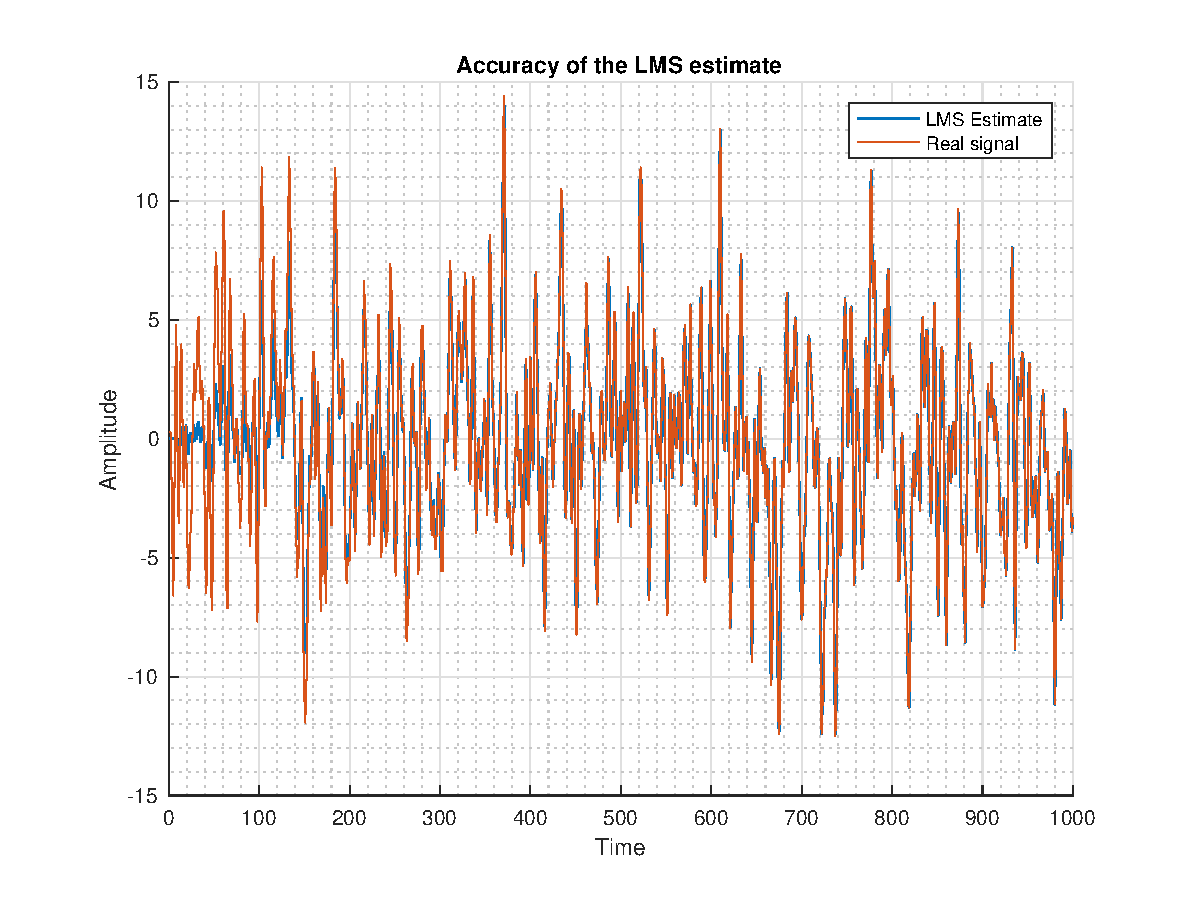
\includegraphics[width = \textwidth]{lms_acc_1}
\caption{$\sigma_N=0.01$}
\label{fig:lms_acc_1}
\end{subfigure}
\begin{subfigure}{0.33\textwidth}
\centering
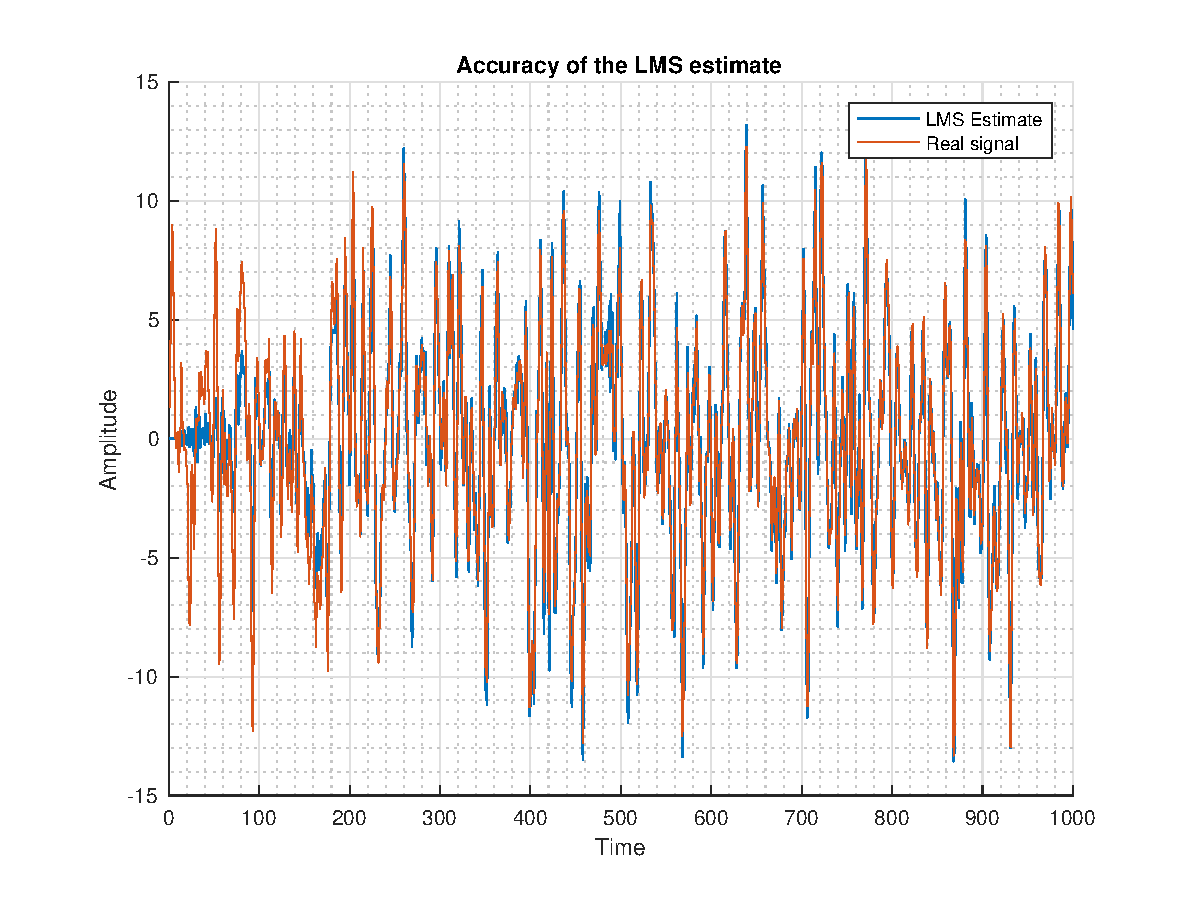
\includegraphics[width = \textwidth]{lms_acc_2}
\caption{$\sigma_N=3.1$}
\label{fig:lms_acc_2}
\end{subfigure}
\caption{\label{fig:lms_accuracy} Comparing the input signal \textbf{x} with the LMS estimate}
\end{figure}


\subsubsection{Time evolution of coefficients}

Figure \ref{fig:lms_error} shows the time evolution of the estimated error squared for adaptive gain $\mu=0.01$, which becomes almost negligible after the 250th sample. Figure \ref{fig:time_evol_g01} shows the time evolution of the optimal coefficients for $\mu=0.01$. The rest of Figure \ref{time_evol} shows the time evolution of optimal coefficients for different values of $\mu$. 

\begin{figure}[h!]
\centering
\begin{subfigure}{0.32\textwidth}
\centering
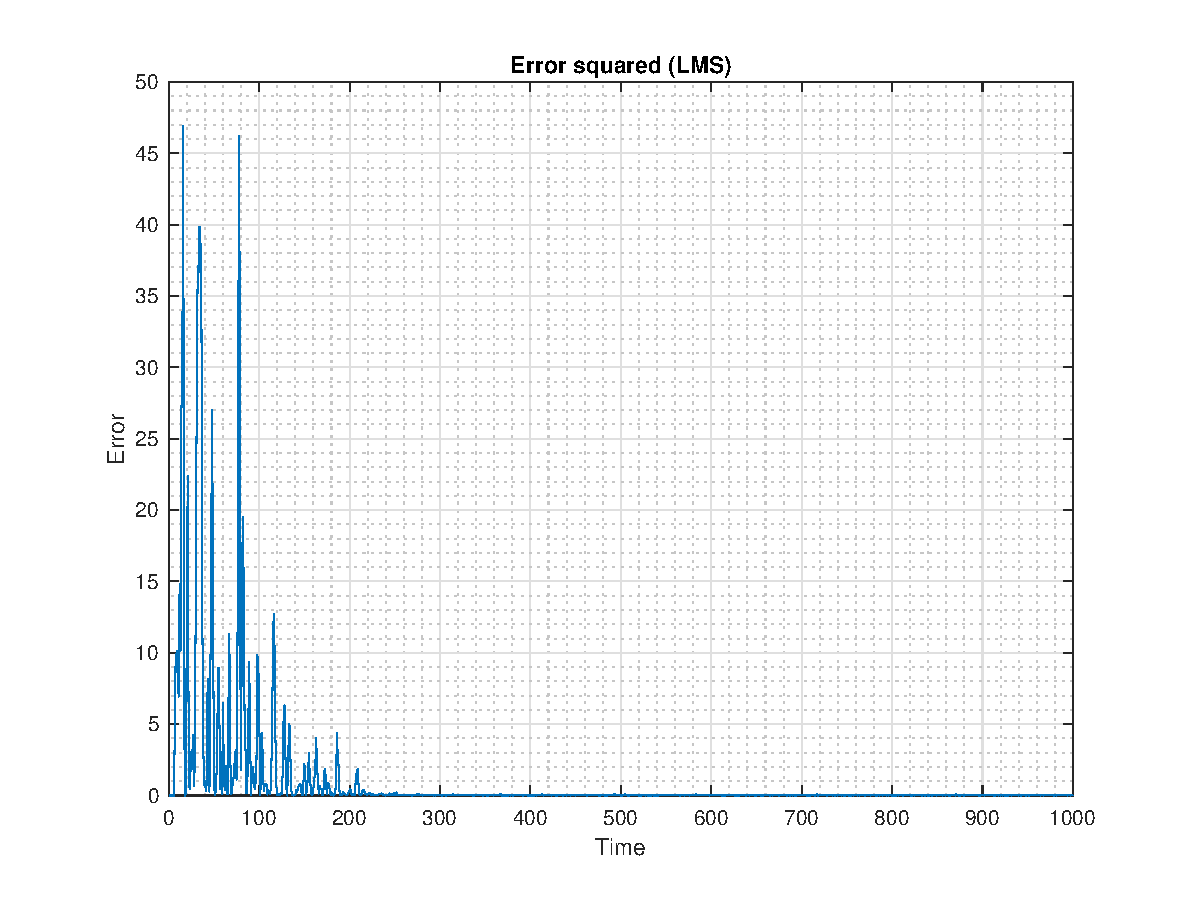
\includegraphics[width = \textwidth]{lms_error}
\caption{Error squared ($\mu=0.01$)}
\label{fig:lms_error}
\end{subfigure}
\begin{subfigure}{0.32\textwidth}
\centering
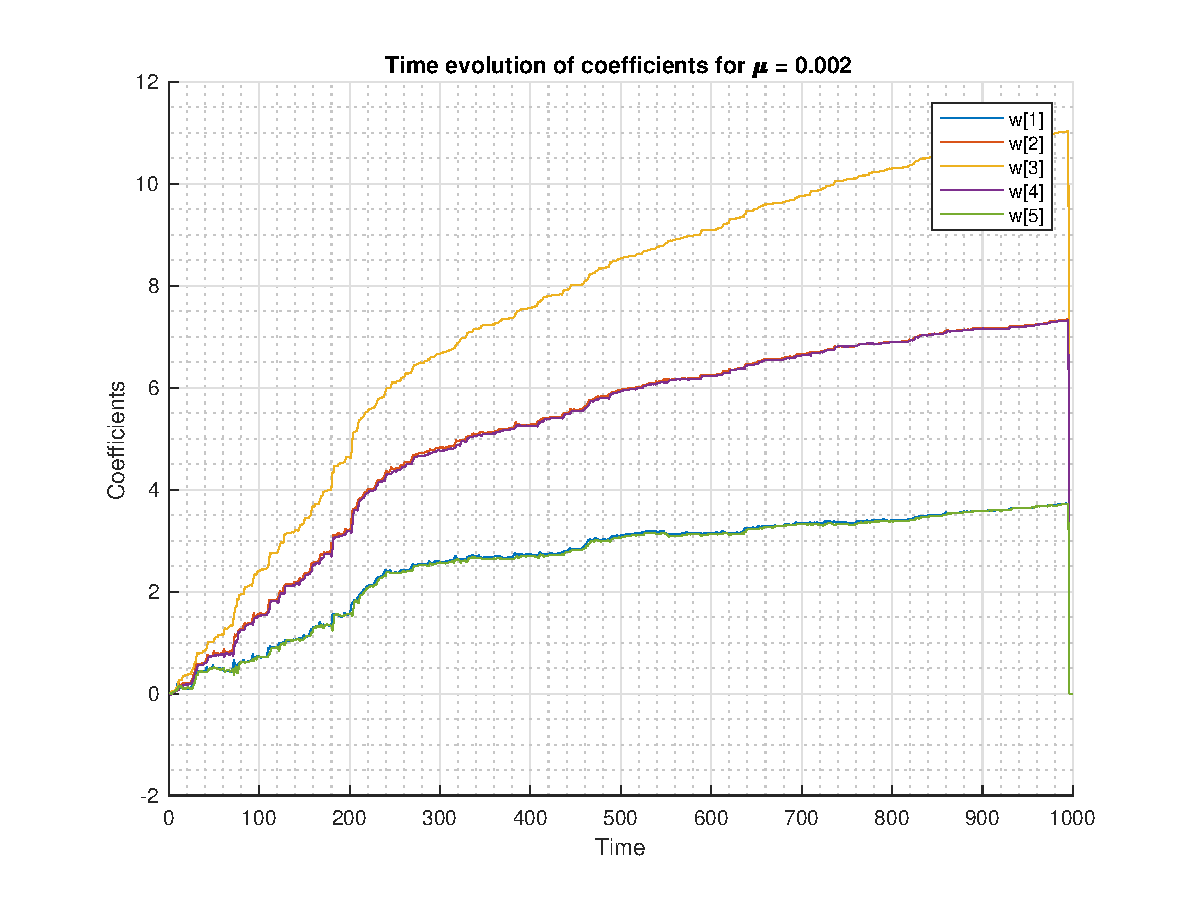
\includegraphics[width = \textwidth]{time_evol_g002}
\caption{Coefficients for $\mu=0.002$}
\label{fig:time_evol_g002}
\end{subfigure}
\begin{subfigure}{0.32\textwidth}
\centering
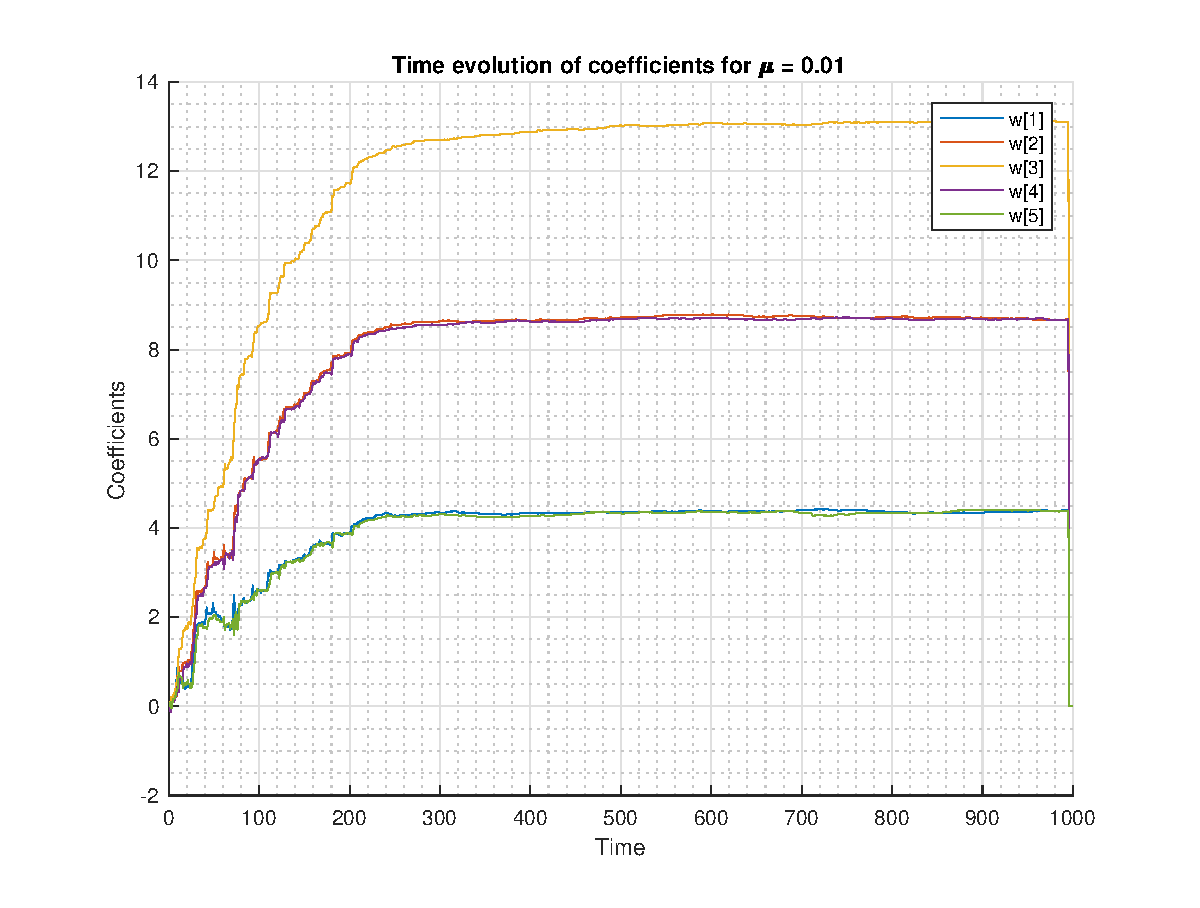
\includegraphics[width = \textwidth]{time_evol_g01}
\caption{Coefficients for $\mu=0.01$}
\label{fig:time_evol_g01}
\end{subfigure}
\begin{subfigure}{0.32\textwidth}
\centering
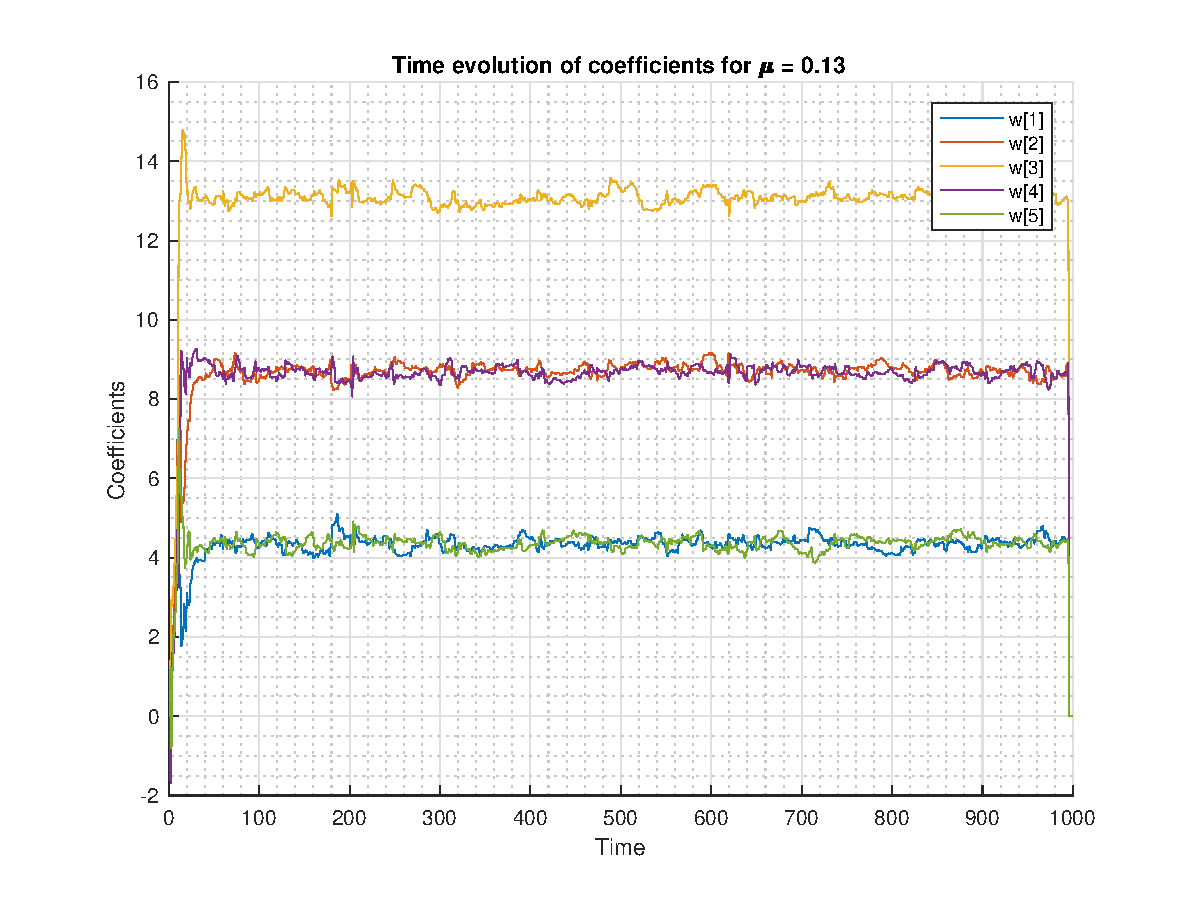
\includegraphics[width = \textwidth]{time_evol_g13}
\caption{Coefficients for $\mu=0.13$}
\label{fig:time_evol_g13}
\end{subfigure}
\begin{subfigure}{0.32\textwidth}
\centering
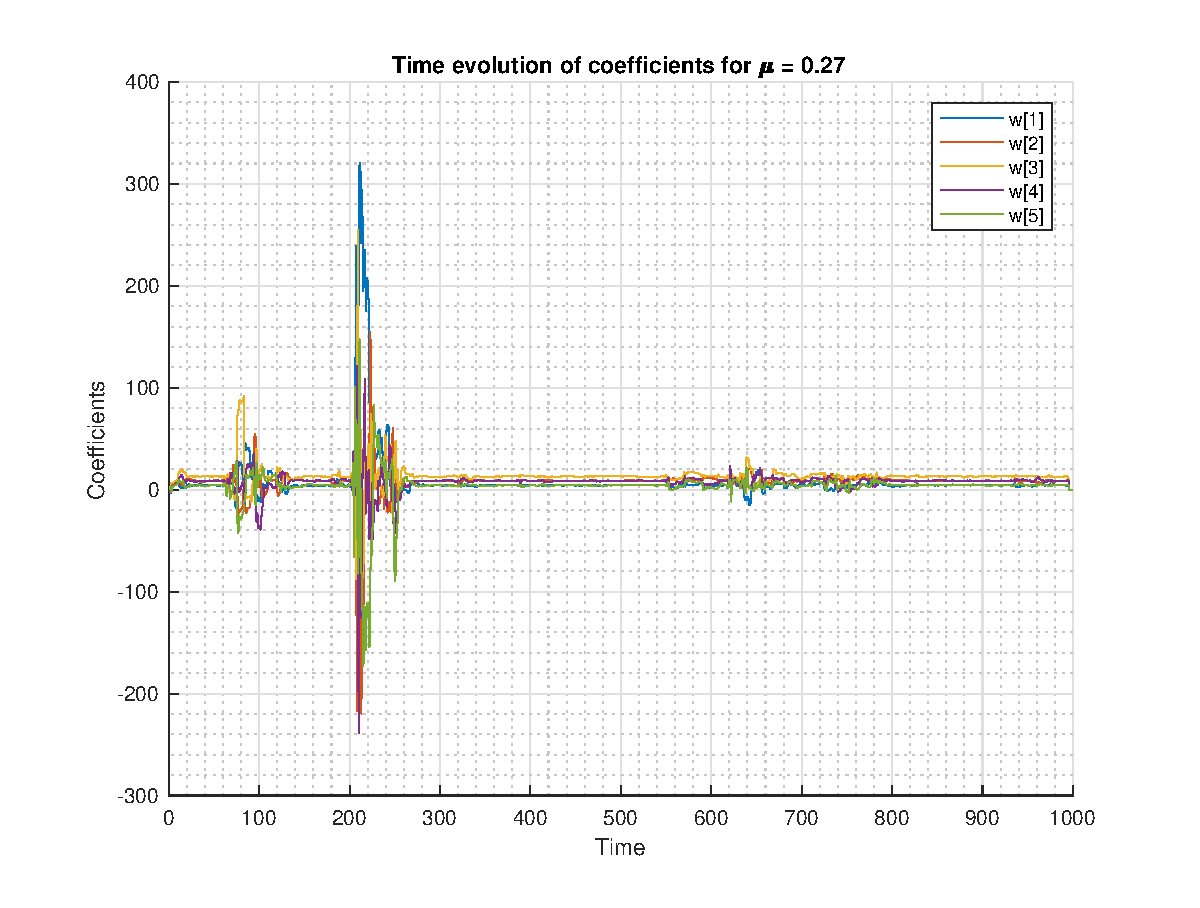
\includegraphics[width = \textwidth]{time_evol_g27}
\caption{Coefficients for $\mu=0.27$}
\label{fig:time_evol_g27}
\end{subfigure}
\begin{subfigure}{0.32\textwidth}
\centering
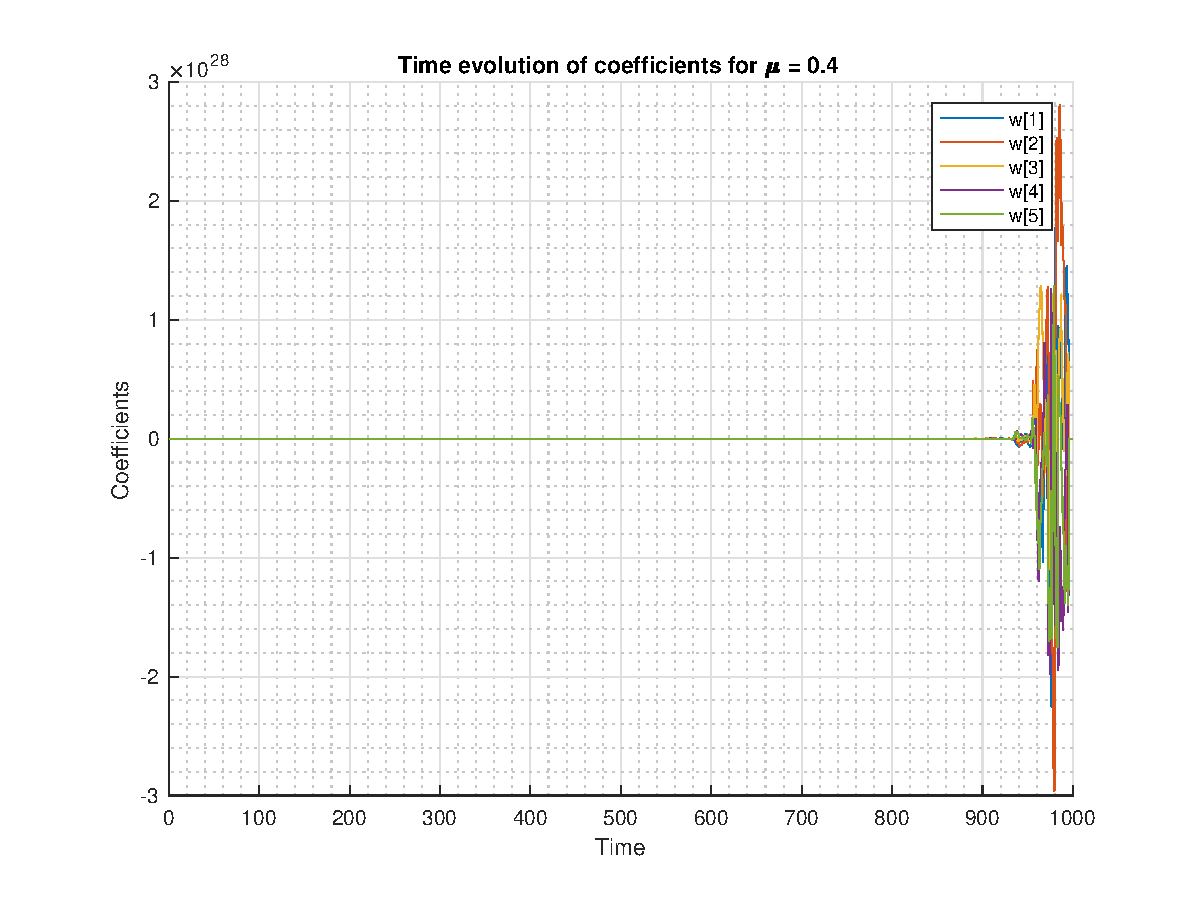
\includegraphics[width = \textwidth]{time_evol_g4}
\caption{Coefficients for $\mu=0.4$}
\label{fig:time_evol_g4}
\end{subfigure}
\caption{Comparing the time evolution of optimal coefficients for different values of adaptive gain $\mu$}
\label{time_evol}
\end{figure}

\pagebreak

Increasing $\mu$ causes the coefficients to converge to their ideal values faster, which in turn causes the error to converge to 0 more quickly. Reducing $\mu$ delays this convergence (see Figure \ref{fig:time_evol_g002}). For low $\mu$, the gradual convergence of the coefficients to their ideal values would make the estimate smoothly converge to the ideal signal. However, increasing $\mu$ beyond a certain point (see Figure \ref{fig:time_evol_g13}) causes the coefficients to diverge from the ideal. The error increases and the estimated coefficients (and hence the estimated signal) completely diverges from the ideal (see Figure \ref{fig:time_evol_g27}).


\subsubsection{Computational complexity of the LMS algorithm}

The complexity can be determined by analyzing the 3 equations that make the LMS algorithm. $w(n+1)=w(n)+\mu e[n]x(n)$ requires $N_w+1$ additions. This is denoted as O($N_w+1$). The transpose in $\hat{y}[n]=w^T(n)x(n)$ would be approximately $O(N_w)$. The product of the $N_w$ by $N_w+1$ matrix with an $N_w+1$ by 1 column would be $O(N_w+1) + O(N_w)$. Calculating the error is a simple subtraction of scalar values and hence does not influence the complexity. Assuming $N_w>>1$, the total complexity is of the order $4O(N_w) \approx O(N_w)$.


\subsection{Gear Shifting}

Gear shifting is a natural extension to the previous exercise. $\mu$ is decreased by 20\% if the new error is lower than the old error, and increased by 20\% in the opposite case. This avoids divergence of the coefficients and hence overshoot of the estimated signal $\hat{y}$. The initial gain is kept small in order to avoid divergence. Figure \ref{fig:lms_gs} shows the faster convergence of coefficients and error for $\mu=0.1$ compared to the standard LMS algorithm.

\begin{figure}[h!]
\centering
\begin{subfigure}{0.33\textwidth}
\centering
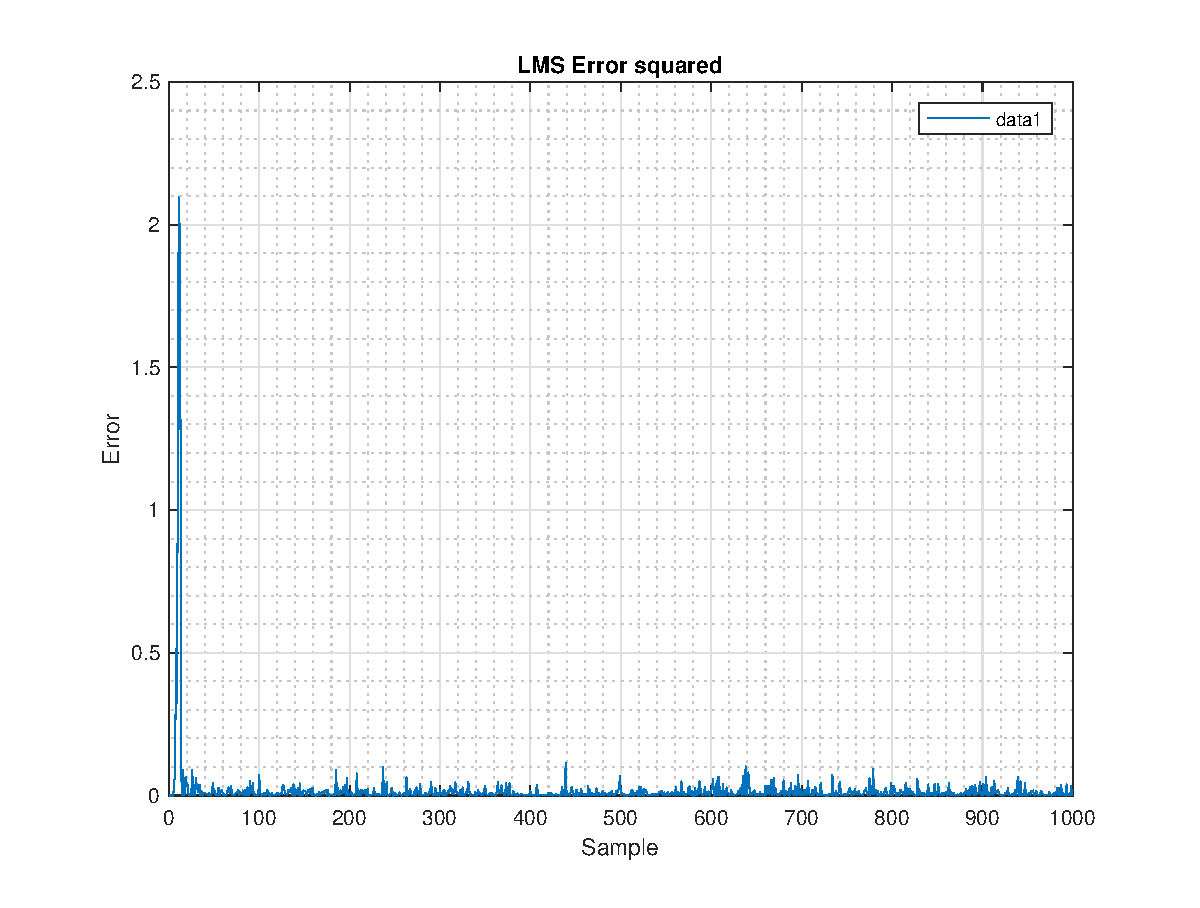
\includegraphics[width = \textwidth]{lms_gs_error}
\caption{Error squared}
\label{fig:lms_gs_error}
\end{subfigure}
\begin{subfigure}{0.33\textwidth}
\centering
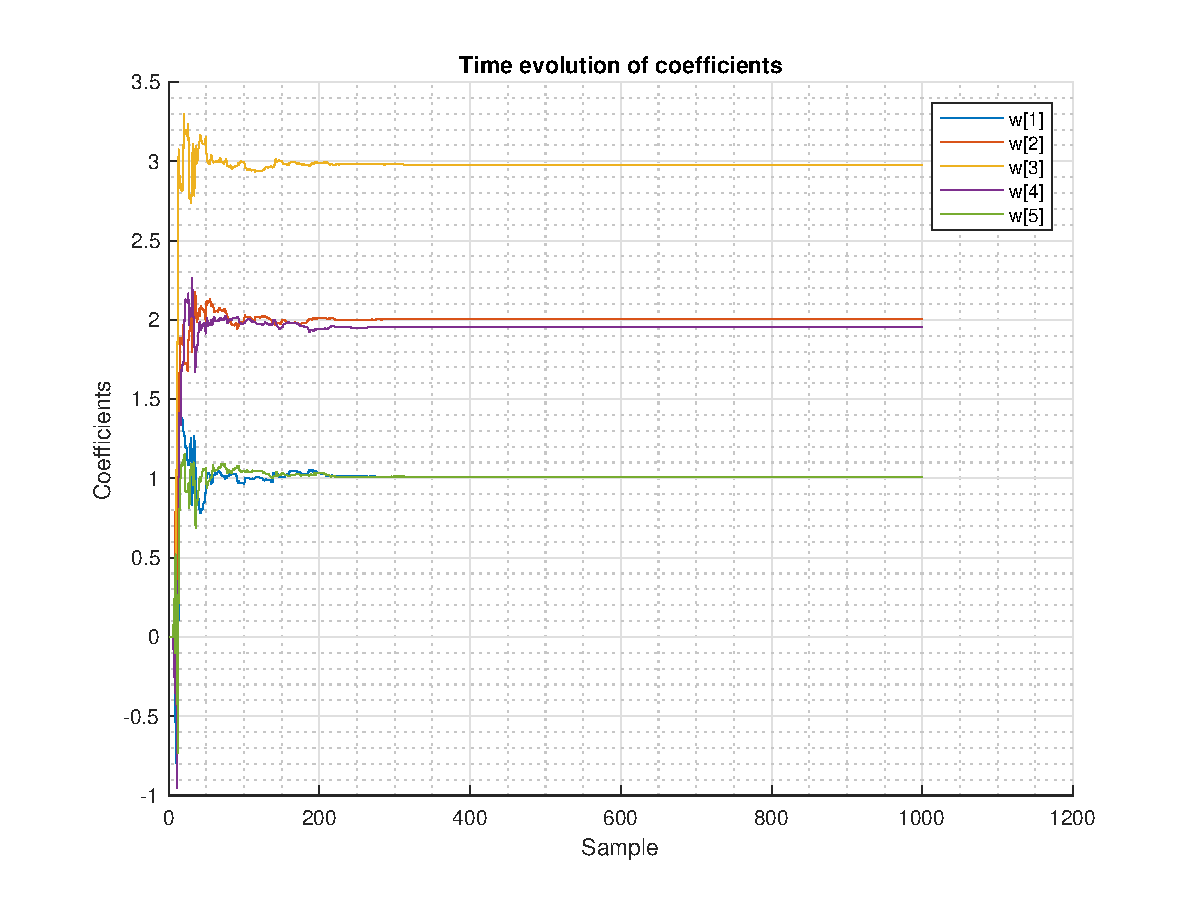
\includegraphics[width = \textwidth]{lms_gs_timeevol}
\caption{Evolution of coefficients}
\label{fig:lms_gs_timeevol}
\end{subfigure}
\caption{\label{fig:lms_gs} Faster convergence using gear shifted LMS algorithm for $\mu=0.1$}
\end{figure}

\pagebreak

\subsection{Identification of AR processes}

\subsubsection{Implementing the given AR model}

Since the given system is an AR(2) process, the LMS algorithm needs to estimate $a_1$ and $a_2$. Figure \ref{fig:ar_g01} shows that the coefficients converge to -0.2 and -0.9. This is because the filter output is defined by:

\begin{equation*}
y(n)=\sum_{i=0}^M b_i x(n-i) - \sum_{j=0}^N a_j x(n-j) = -0.9x(n-1) - 0.2x(n-2)
\end{equation*}


\subsubsection{Evolution of AR coefficients for different gains}

The plots in Figure \ref{ar_gain} have been extended to 5000 samples so that the convergence is clear. The convergence is too slow for $\mu=0.001$ and the estimate is too distorted for $\mu=0.1$. There is a good balance between accuracy and speed of convergence at $\mu=0.01$.

\begin{figure}[h!]
\centering
\begin{subfigure}{0.33\textwidth}
\centering
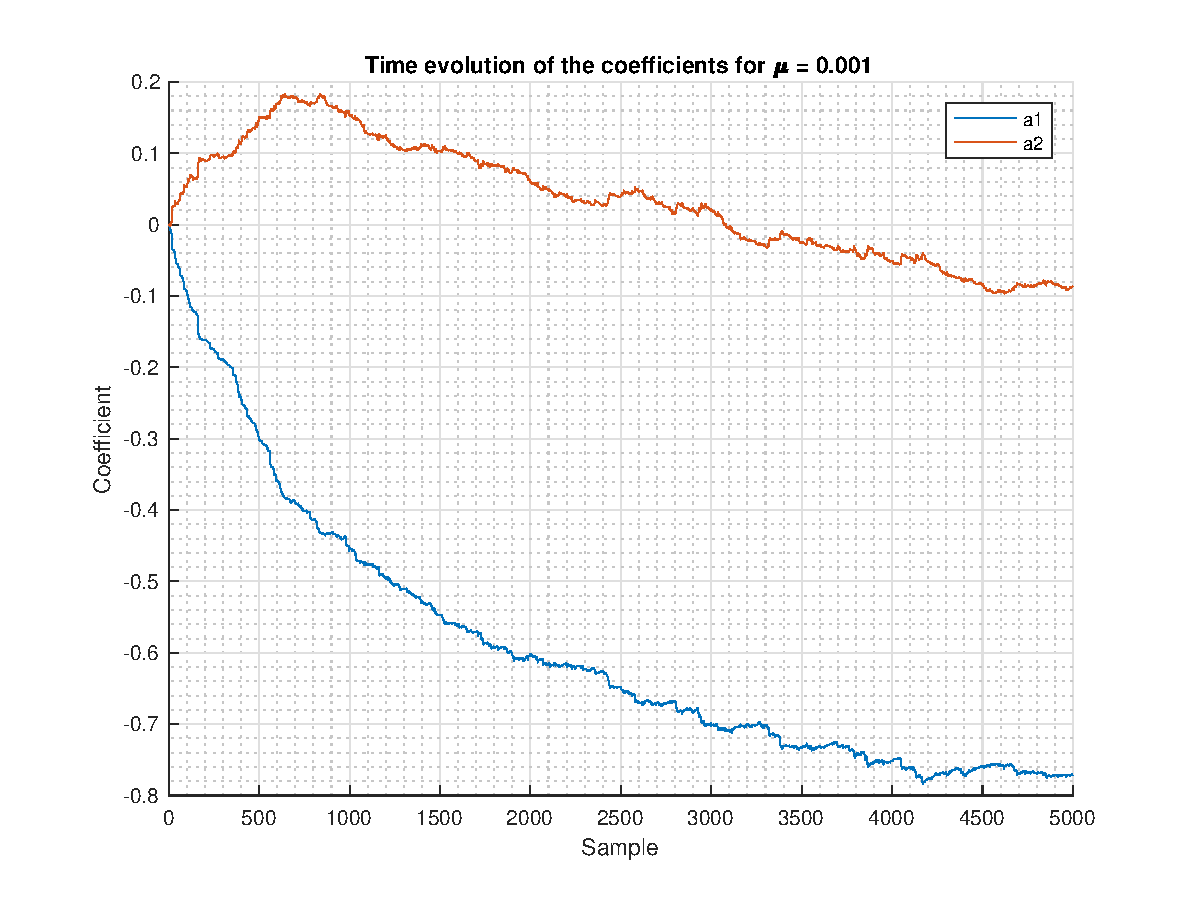
\includegraphics[width = \textwidth]{ar_g001}
\caption{AR coefficients for $\mu=0.001$}
\label{fig:ar_g001}
\end{subfigure}
\begin{subfigure}{0.33\textwidth}
\centering
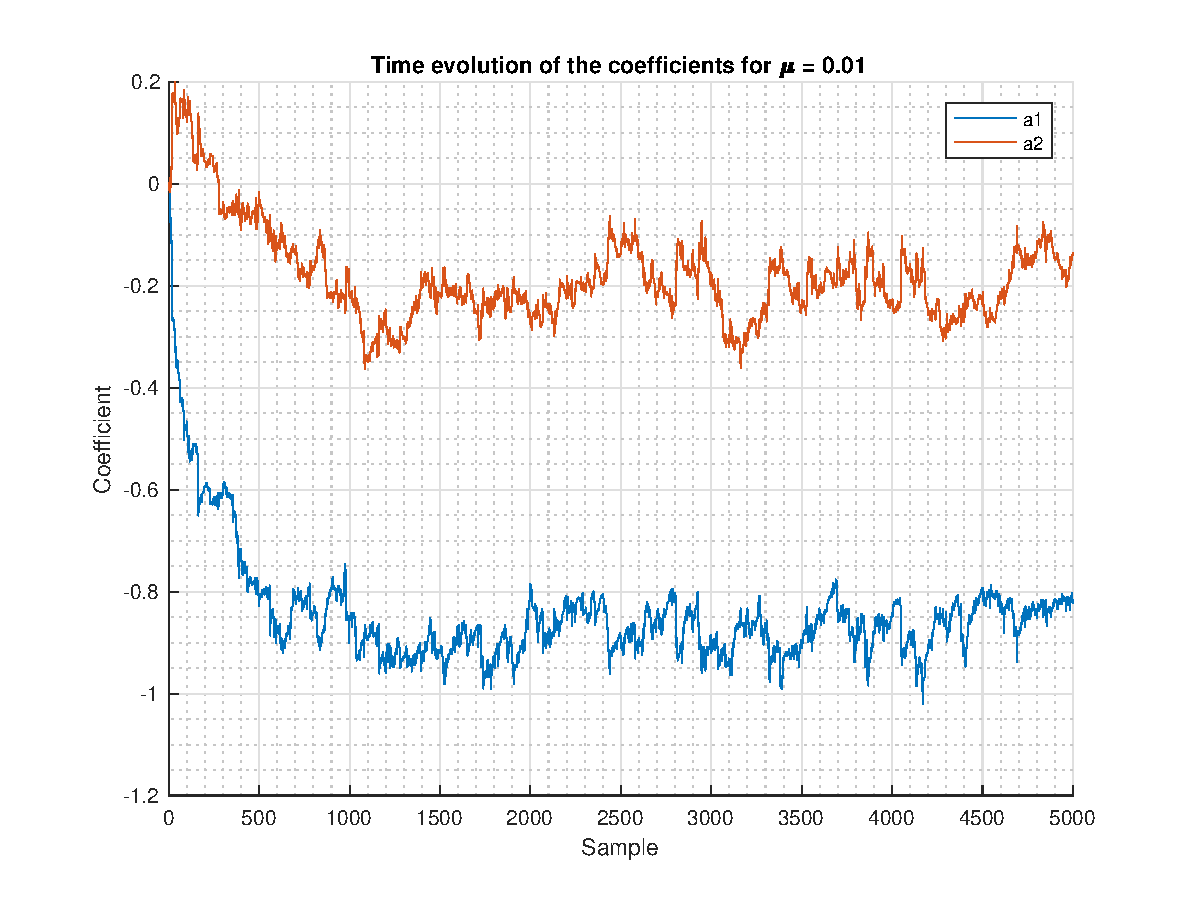
\includegraphics[width = \textwidth]{ar_g01}
\caption{AR coefficients for $\mu=0.01$}
\label{fig:ar_g01}
\end{subfigure}
\begin{subfigure}{0.33\textwidth}
\centering
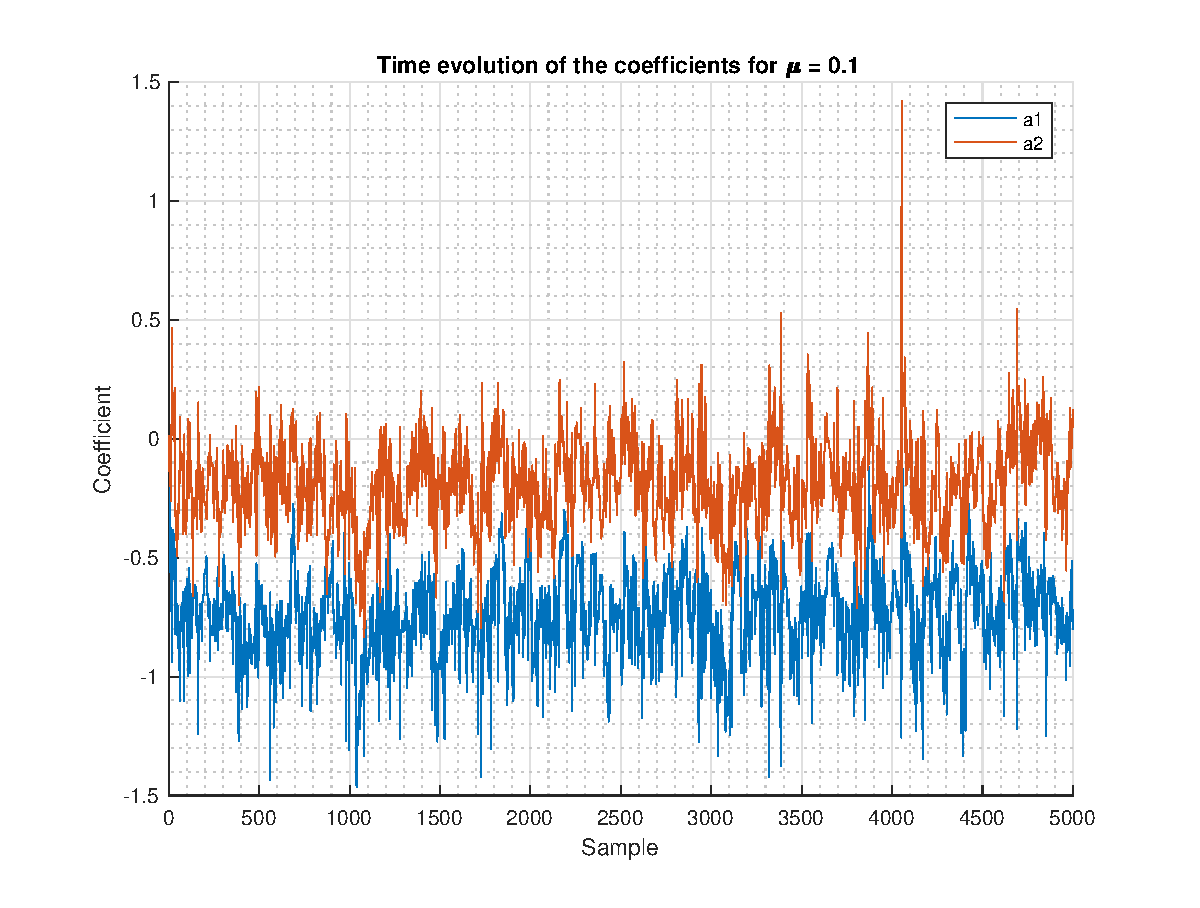
\includegraphics[width = \textwidth]{ar_g1}
\caption{AR coefficients for $\mu=0.1$}
\label{fig:ar_g1}
\end{subfigure}
\begin{subfigure}{0.33\textwidth}
\centering
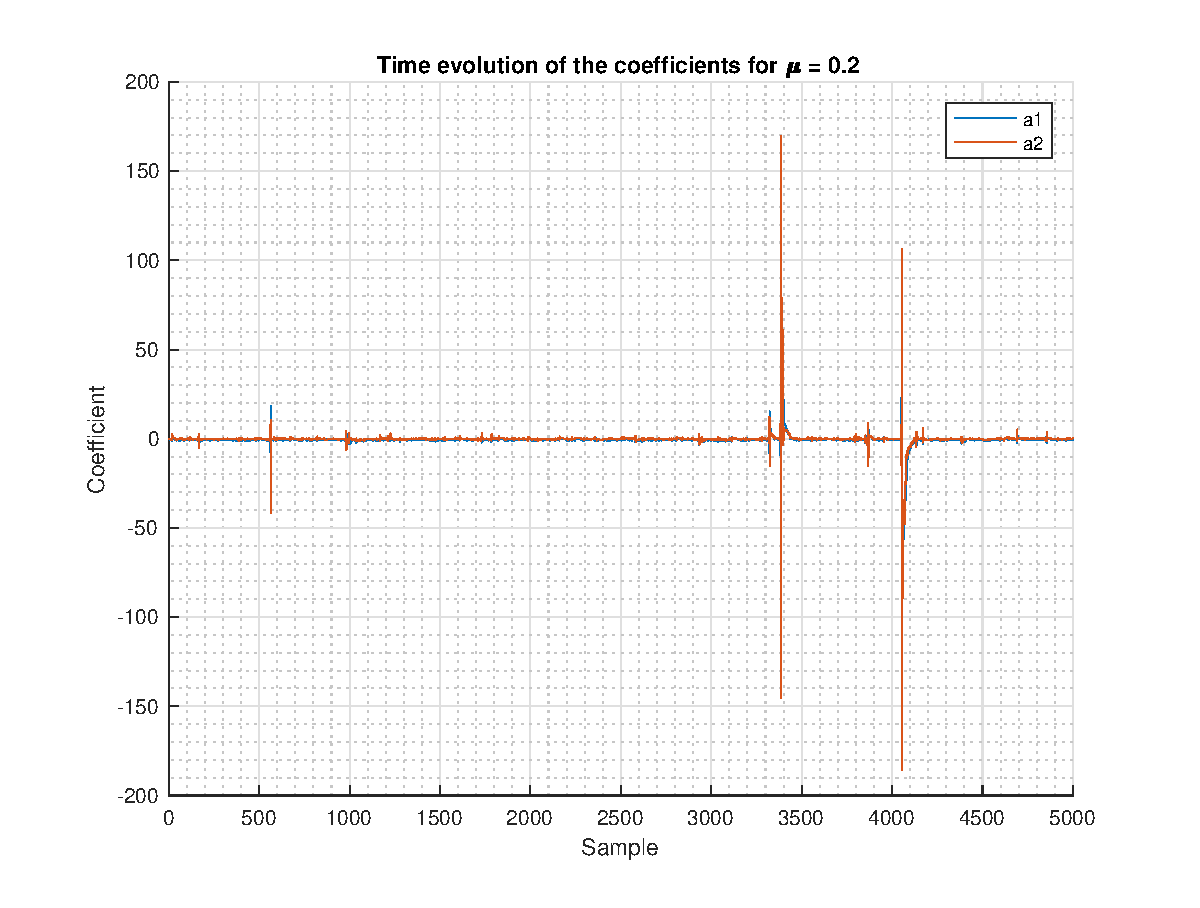
\includegraphics[width = \textwidth]{ar_g2}
\caption{AR coefficients for $\mu=0.2$}
\label{fig:ar_g2}
\end{subfigure}
\caption{Evolution of AR coefficients $a_1$ and $a_2$ for different values of $\mu$}
\label{ar_gain}
\end{figure}

\pagebreak

\subsection{Speech Recognition}

\subsubsection{Testing the predictor performance}

The model proposed in the earlier section is now used to estimate the best prediction order for 5 pieces of audio data - "e", "a", "s", "t", and "x". We use the MDL and AIC to determine the orders, and the results are tabulated in Table \ref{tab:speech_mdl}.

\begin{table}[h!]
\centering
\begin{tabular}{|c|c|c|c|c|c|}
\hline
\multirow{2}{*}{Criterion} & \multicolumn{5}{c|}{Recommended Order} \\ \cline{2-6} 
                           & e      & a     & s     & t     & x     \\ \hline
MDL                        & 4      & 7     & 5     & 4     & 5     \\ \hline
AIC                        & 5      & 23     & 6     & 4     & 8     \\ \hline
\end{tabular}
\caption{Recommended model order for each letter's audio signal}
\label{tab:speech_mdl}
\end{table}

The calculations above use 1000 samples, a sampling frequency of 441 kHz, an adaption gain of 0.5, and a filter order of 20. The low $\mu$ and high order have been chosen to ensure accuracy. Gear shifting is not recommended in this case since the speech signal is non-stationary, and the gear shifting algorithm would introduce errors in the estimates since it is strictly meant for stationary processes. Increasing the adaptation gain beyond 0.8 causes diversion in the estimates.

\begin{figure}[h!]
\centering
\begin{subfigure}{0.24\textwidth}
\centering
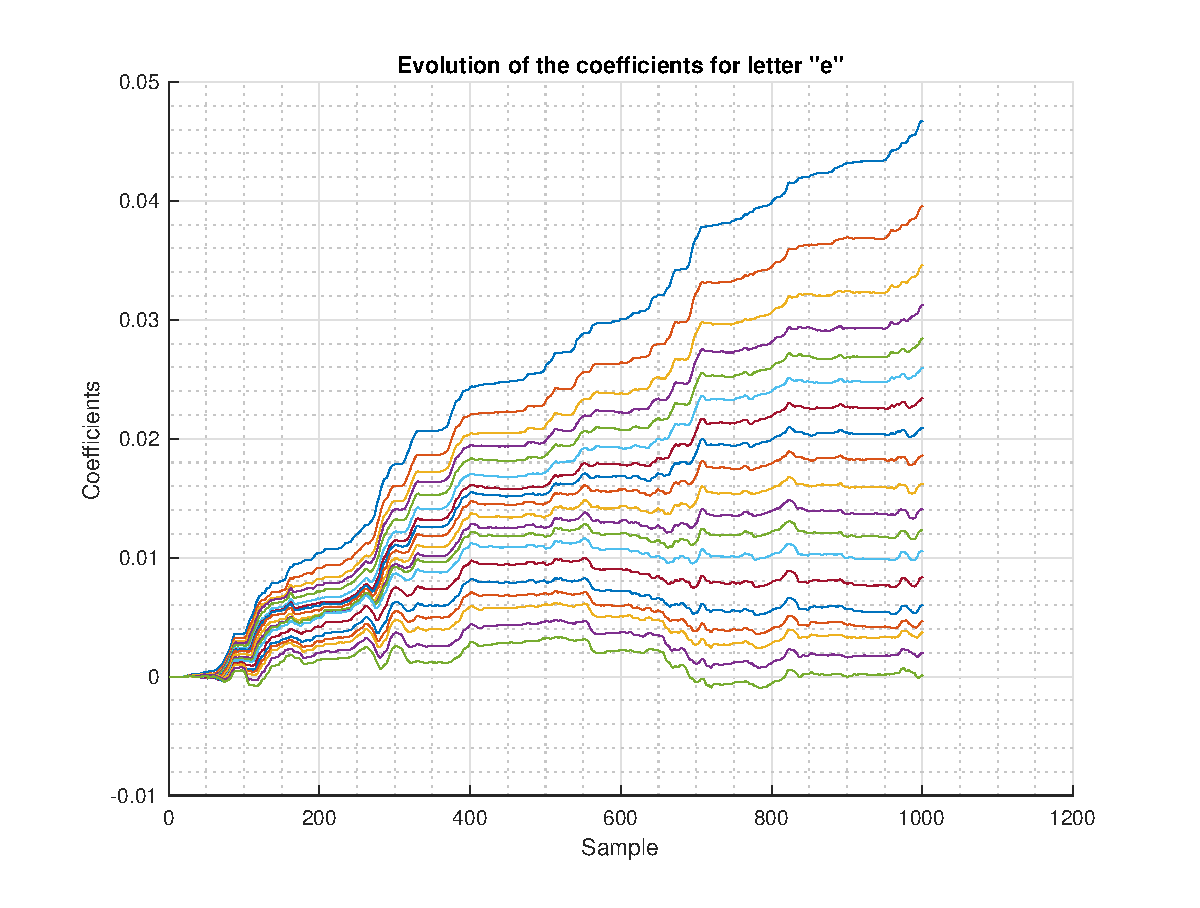
\includegraphics[width = \textwidth]{speech_e}
\caption{Coefficients for "e"}
\label{fig:speech_e}
\end{subfigure}
\begin{subfigure}{0.24\textwidth}
\centering
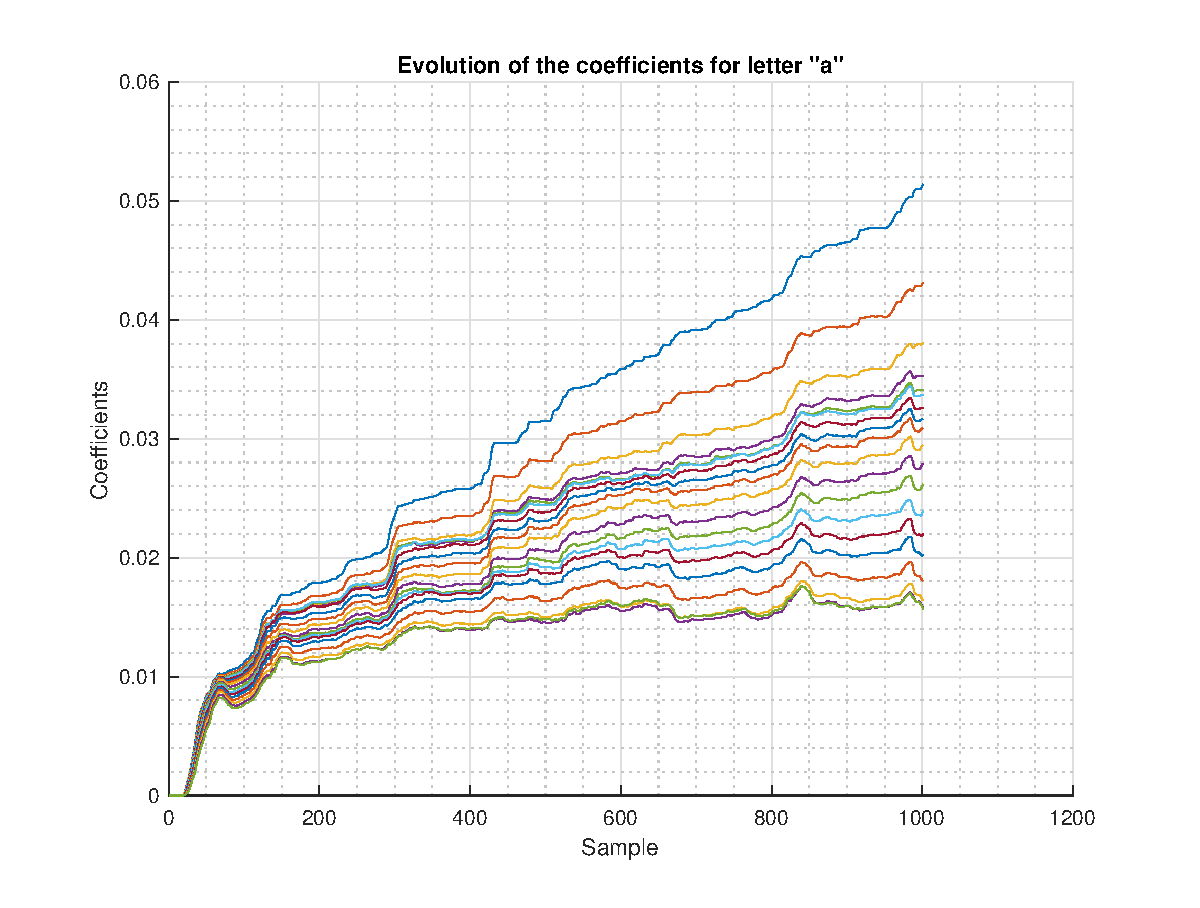
\includegraphics[width = \textwidth]{speech_a}
\caption{Coefficients for "a"}
\label{fig:speech_a}
\end{subfigure}
\begin{subfigure}{0.24\textwidth}
\centering
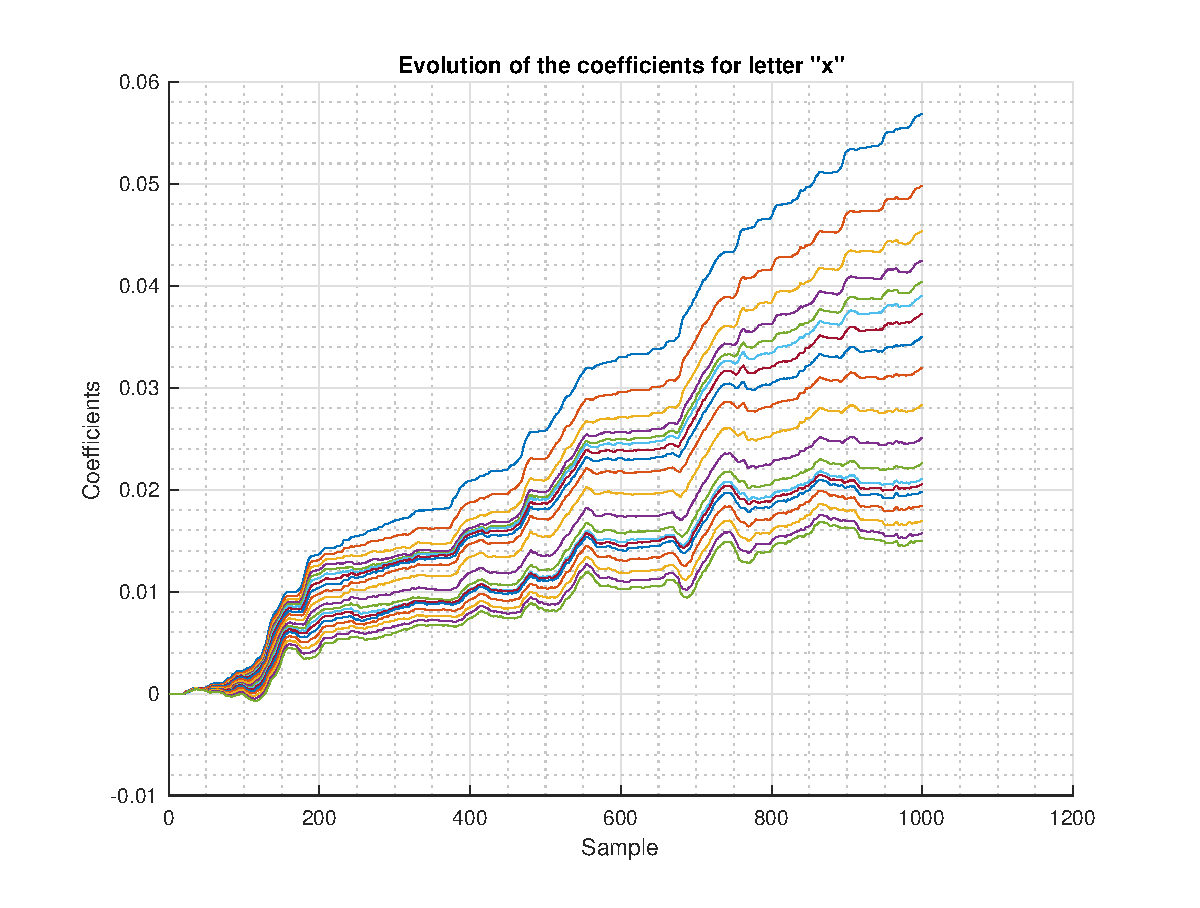
\includegraphics[width = \textwidth]{speech_x}
\caption{Coefficients for "x"}
\label{fig:speech_x}
\end{subfigure}
\begin{subfigure}{0.24\textwidth}
\centering
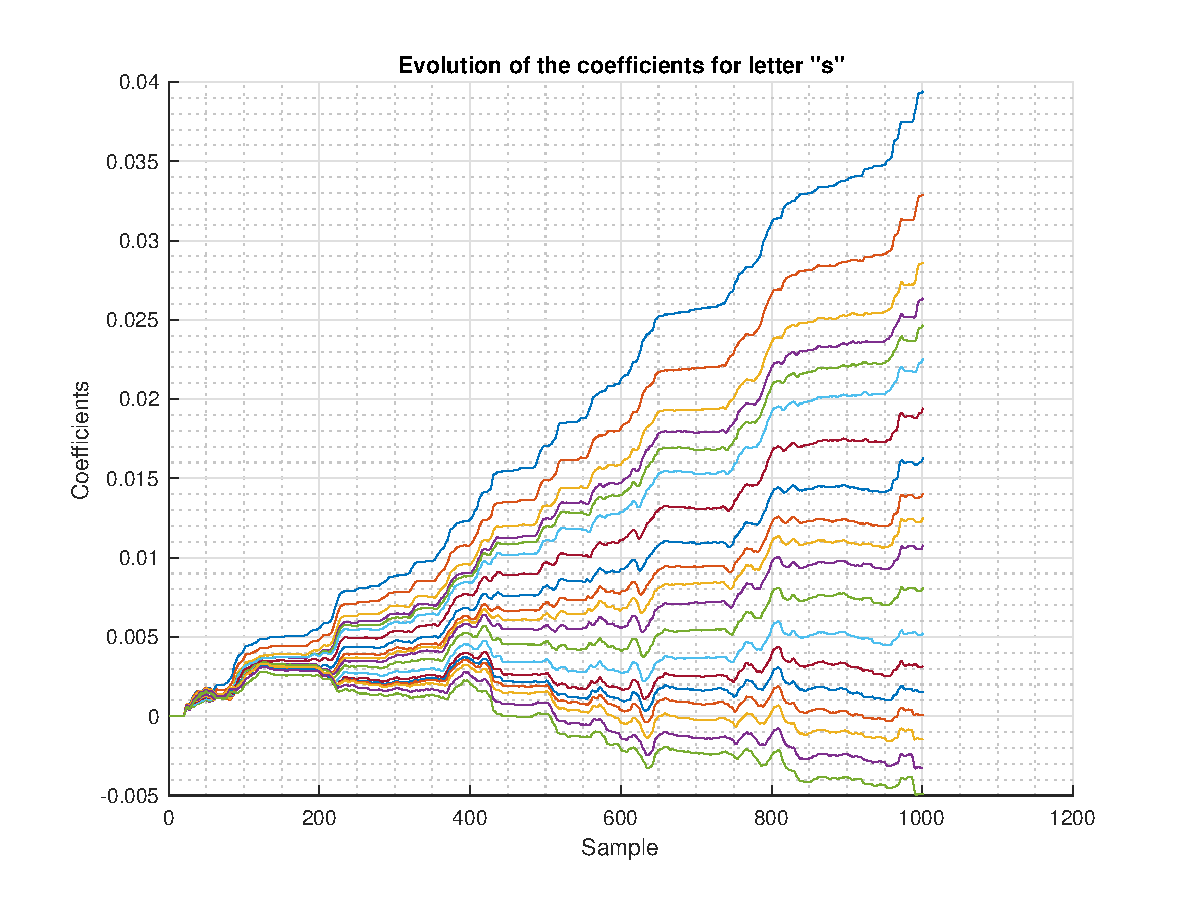
\includegraphics[width = \textwidth]{speech_s}
\caption{Coefficients for "s"}
\label{fig:speech_s}
\end{subfigure}
\caption{Convergence of coefficients for the audio signals}
\label{fig:speech_converge}
\end{figure}


\subsubsection{The optimal filter length}

The optimal filter length could be found by looking for the combination of $\mu$ and p that gives the maximum $R_p$. This must also be balanced with the constraint on computational complexity, since higher orders require more mathematical operations. Table \ref{tab:filter_len} shows the variation in prediction gain for the audio signal "e" when adaptation gain and filter order are changed.\\

Every person's speech can be modeled uniquely depending on the specific frequency components in their voice. $R_p$ peaks at p=5 for $\mu=0.1$, which implies that a 5th order system is optimal for modeling my voice. The estimated orders become distorted for $\mu>0.8$, so the trends for $\mu=1,2$ may be ignored for the purpose of this analysis.

\begin{table}[h!]
\centering
\begin{tabular}{|c|c|c|c|c|c|}
\hline
           & p=20  & p=15  & p=10  & p=5   & p=1   \\ \hline
$\mu=0.01$ & 25.9189 & 25.9321 & 25.9413 & 25.9484 & 25.9654 \\ \hline
$\mu=0.1$  & 25.9940 & 26.1359 & 26.2291 & 26.2565 & 26.2603 \\ \hline
$\mu=1$    & 27.6064 & 27.6103 & 27.5602 & 27.1570 & 26.0351 \\ \hline
$\mu=2$    & 28.4507 & 28.4430 & 28.4166 & 28.0057 & 26.0278 \\ \hline
\end{tabular}
\caption{Trends in prediction gain for "e" across filter order and adaptation gain}
\label{tab:filter_len}
\end{table}


\pagebreak


\subsubsection{Assessing the predictor performance at $F_s$ = 16 kHz}

Tables \ref{tab:pred_gain} and \ref{tab:speech_mdl_16k} illustrate the difference in performance for sampling at 44.1 kHz and 16 kHz. There is a higher prediction gain at 44.1 kHz and lower recommended model orders for "e", "s", and "x". This is indicative of better performance. However, the lower sampling rate causes oscillations in the recommended model orders.\\ 

Higher sampling frequency reduces the quantization error since each sample covers a smaller time frame. For a lower sampling rate, the AR process would have to adapt to a wider range of coefficients since the audio signal is not stationary. Increasing the number of samples would compensate for these errors and would allow a lower value of adaptation gain for stable AR coefficients.

\begin{table}[h!]
\centering
\begin{tabular}{|c|c|c|c|c|c|}
\hline
Sampling Frequency & e         & a         & s         & t         & x         \\ \hline
44.1 kHz           & 25.841873 & 23.636714 & 25.282723 & 20.336425 & 20.182098 \\ \hline
16 kHz             & 25.480873 & 24.956100 & 21.369334 & 21.895127 & 18.847481 \\ \hline
\end{tabular}
\caption{Comparing the prediction gain for sampling at 44.1 kHz and 16 kHz}
\label{tab:pred_gain}
\end{table}


\begin{table}[h!]
\centering
\begin{tabular}{|c|c|c|c|c|c|}
\hline
\multirow{2}{*}{Criterion} & \multicolumn{5}{c|}{Recommended Order} \\ \cline{2-6} 
                           & e      & a     & s     & t     & x     \\ \hline
MDL                        & 8      & 4     & 4     & 21     & 4     \\ \hline
AIC                        & 22      &4     & 21     & 21     & 4     \\ \hline
\end{tabular}
\caption{Recommended model order for each letter's audio signal using $F_s$ = 16 kHz}
\label{tab:speech_mdl_16k}
\end{table}

\begin{figure}[h!]
\centering
\begin{subfigure}{0.33\textwidth}
\centering
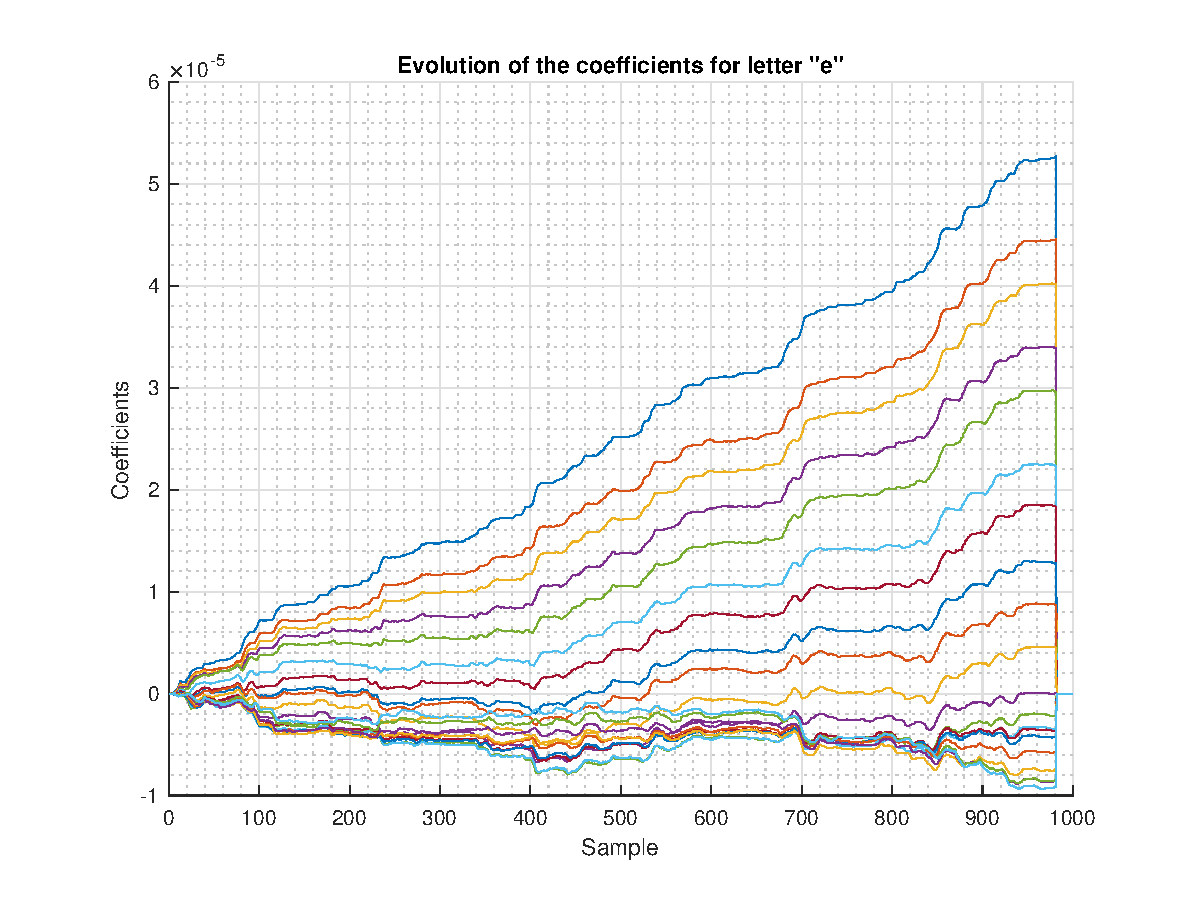
\includegraphics[width = \textwidth]{speech_e_16k}
\caption{$F_s$=16 kHz, $N=1000$, $\mu=0.5$}
\label{fig:speech_e_16k}
\end{subfigure}
\begin{subfigure}{0.33\textwidth}
\centering
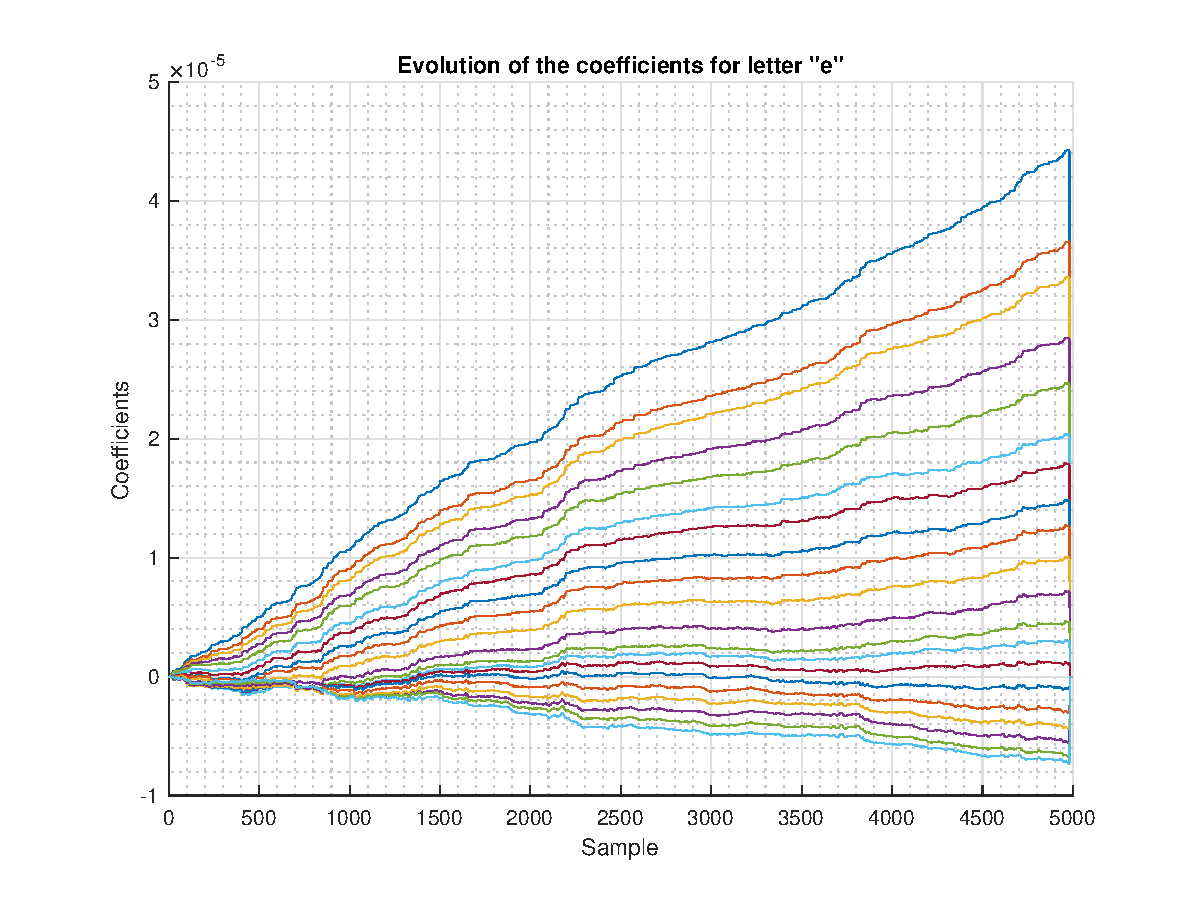
\includegraphics[width = \textwidth]{speech_e_16k_2}
\caption{$F_s$=16 kHz, $N=5000$, $\mu=0.1$}
\label{fig:speech_e_16k_2}
\end{subfigure}
\caption{Improved convergence and stability for coefficients of "e" by increasing number of samples}
\label{speech_e_16k_comp}
\end{figure}


\pagebreak

\subsection{Computational complexity of sign algorithms}

Figure \ref{fig:salg_ar} shows that while the signed LMS algorithms converge to the necessary values (-0.2 and -0.9) faster than the standard LMS, they are much more oscillatory after convergence. Of the signed algorithms, the signed regressor is the slowest to converge but shows the least variance. The sign-sign algorithms shows the largest variance and converges slower than the signed error algorithm.

\begin{figure}[h!]
\centering
\begin{subfigure}{0.33\textwidth}
\centering
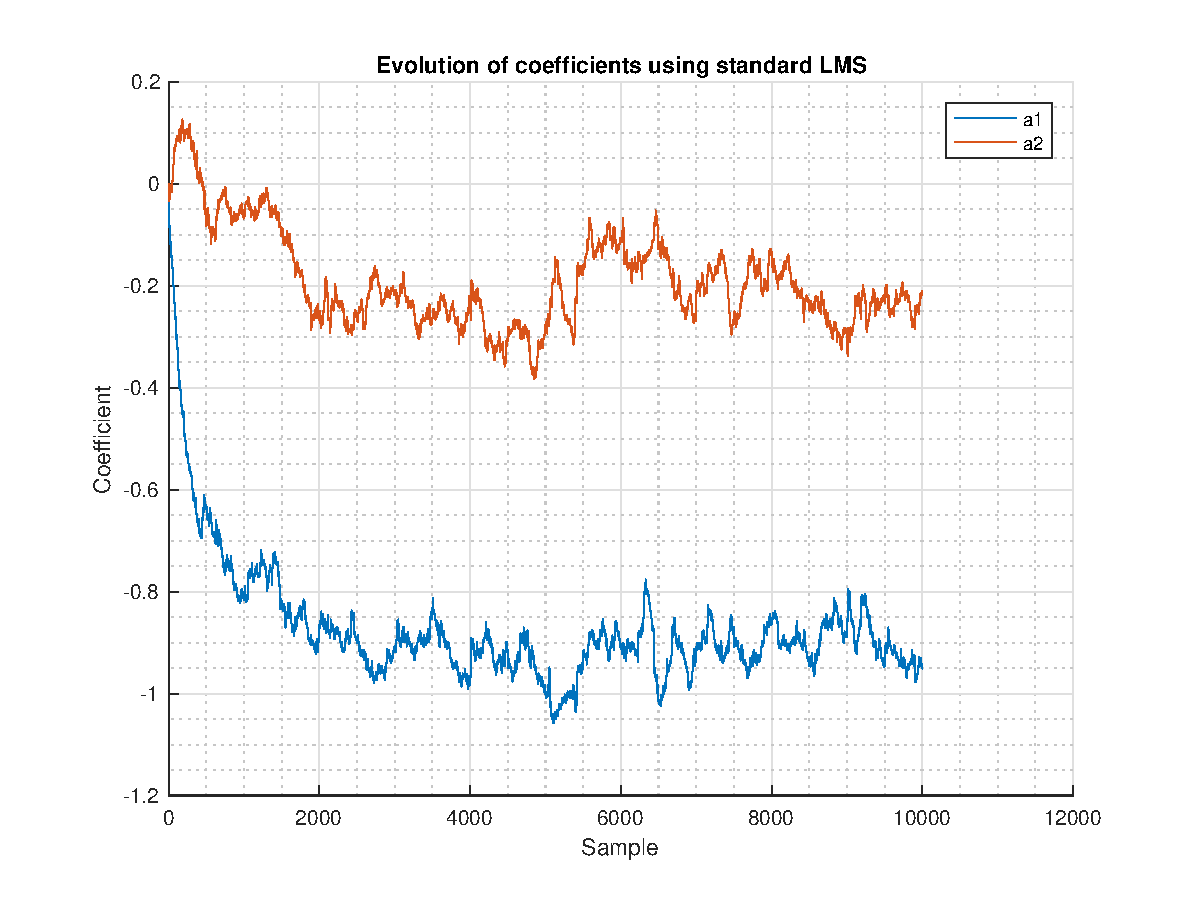
\includegraphics[width = \textwidth]{salg_lms_ar}
\caption{Standard LMS}
\label{fig:salg_lms_ar}
\end{subfigure}
\begin{subfigure}{0.33\textwidth}
\centering
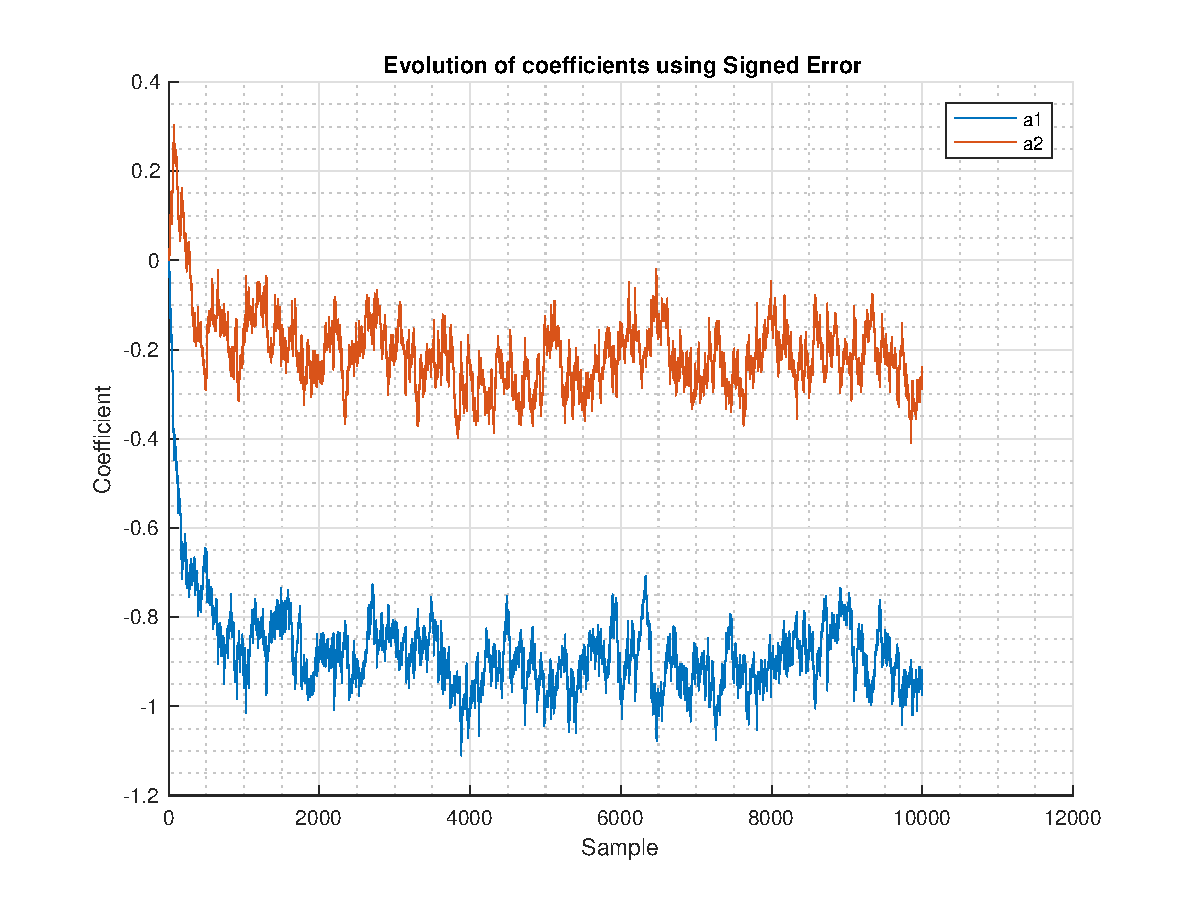
\includegraphics[width = \textwidth]{salg_signerr_ar}
\caption{Signed error}
\label{fig:salg_signerr_ar}
\end{subfigure}
\begin{subfigure}{0.33\textwidth}
\centering
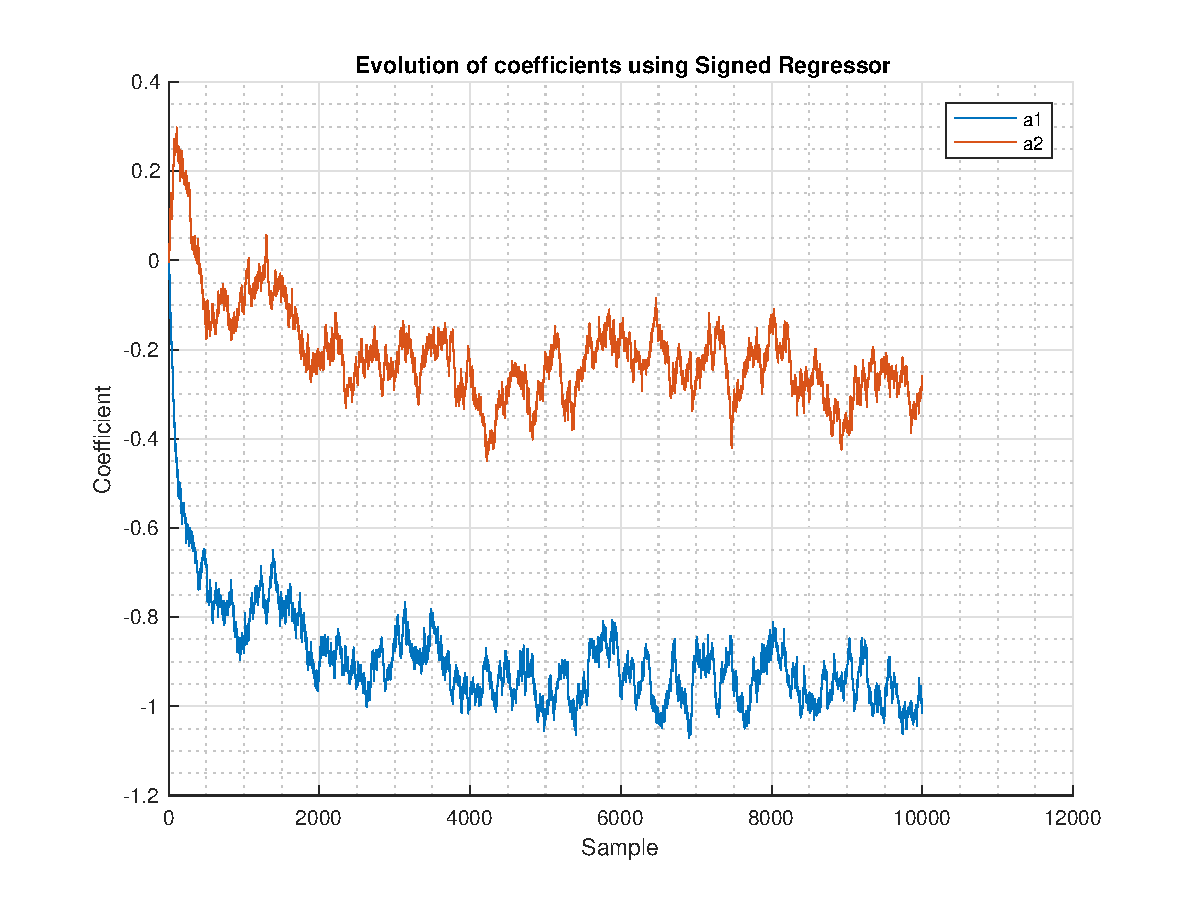
\includegraphics[width = \textwidth]{salg_regressor_ar}
\caption{Signed regressor}
\label{fig:salg_regressor_ar}
\end{subfigure}
\begin{subfigure}{0.33\textwidth}
\centering
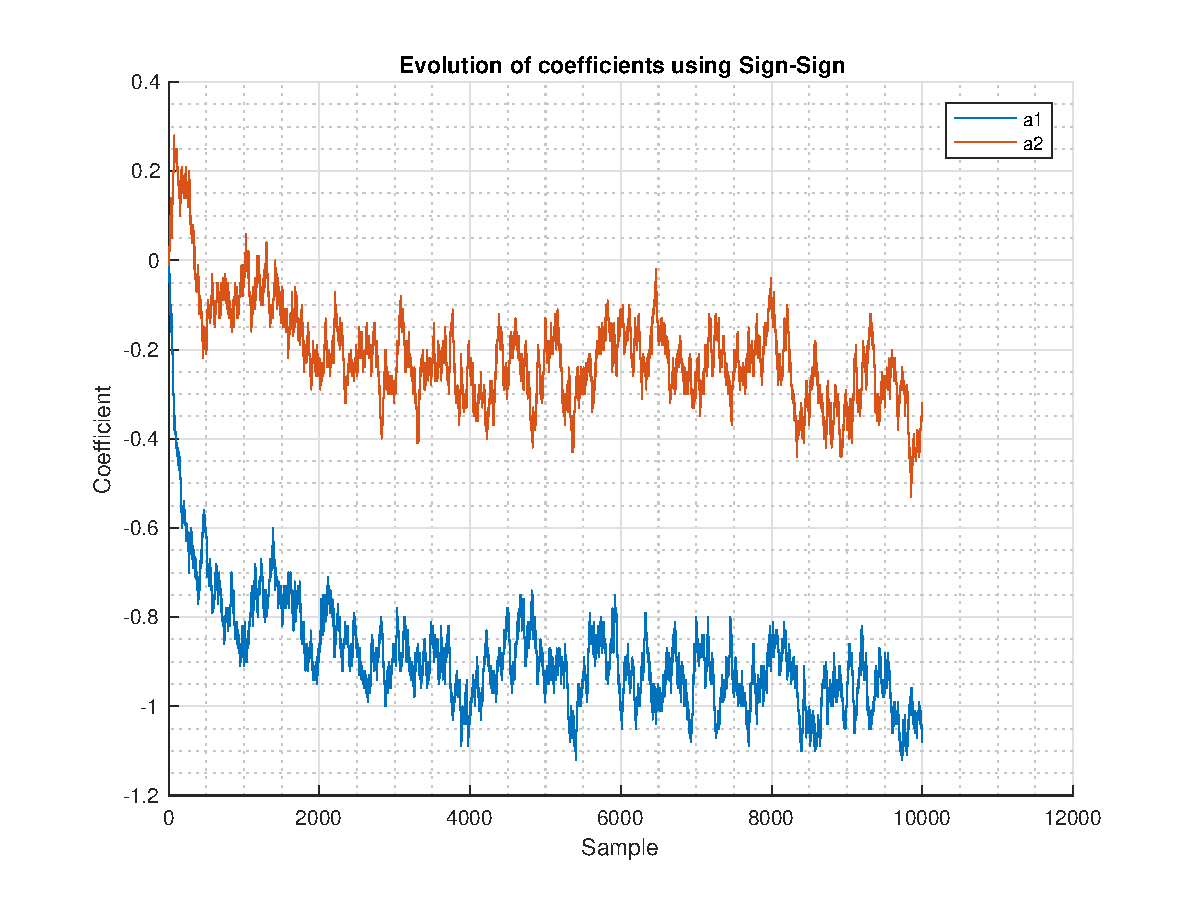
\includegraphics[width = \textwidth]{salg_signsign_ar}
\caption{Sign Sign}
\label{fig:salg_signsign_ar}
\end{subfigure}
\caption{Comparing the performance of signed LMS algorithms for AR prediction}
\label{fig:salg_ar}
\end{figure}


Figure \ref{fig:salg_sp} shows the performance of the signed algorithms on the audio for letter "a". Since the LMS algorithm cannot be applied to speech which is non-stationary, the model orders recommended would be inaccurate. Nevertheless, it is worth noting that the rate of convergence for the standard LMS is lower than that of the signed error and signed regressor. The LMS, signed error and signed regressor recommend identical model orders, while the sign-sign algorithm has skewed predictions.


\begin{figure}[h!]
\centering
\begin{subfigure}{0.24\textwidth}
\centering
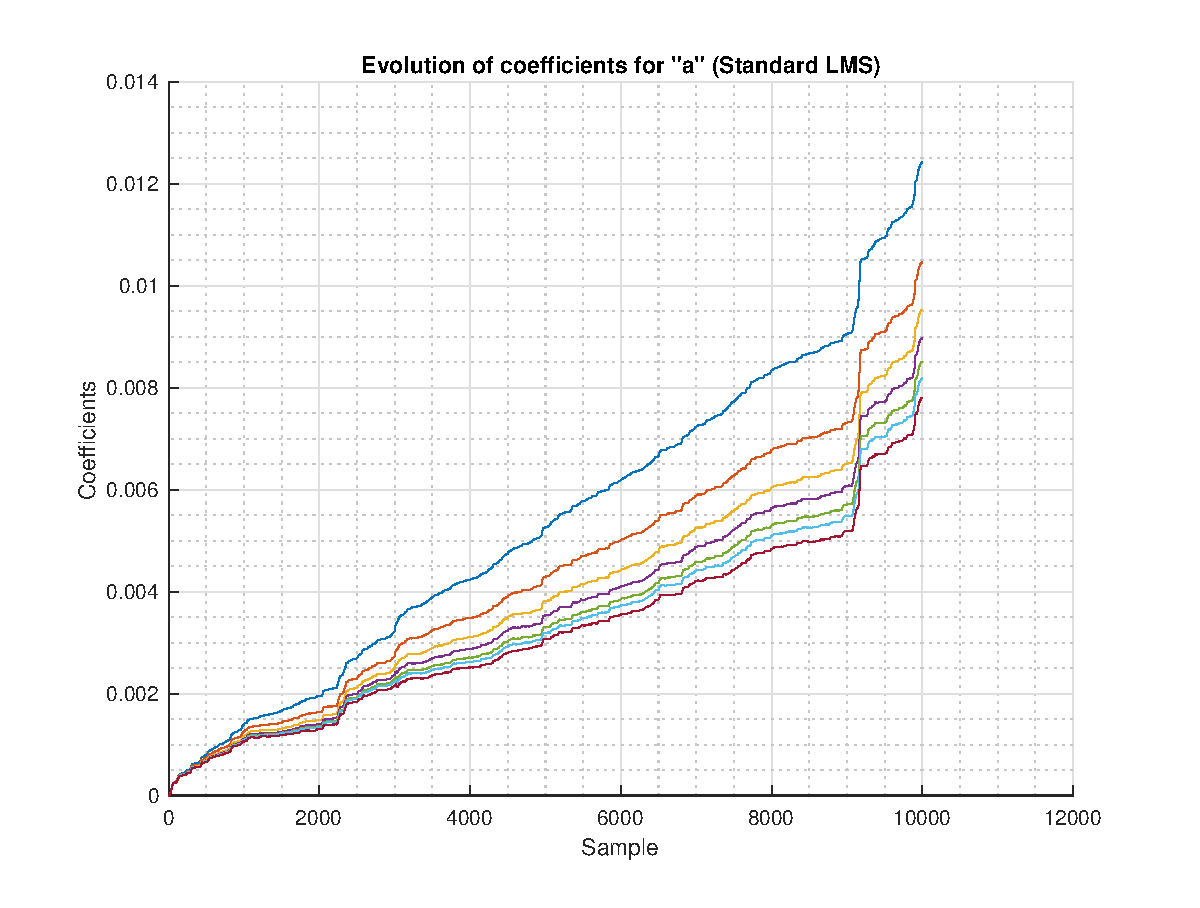
\includegraphics[width = \textwidth]{salg_lms_sp}
\caption{Standard LMS}
\label{fig:salg_lms_sp}
\end{subfigure}
\begin{subfigure}{0.24\textwidth}
\centering
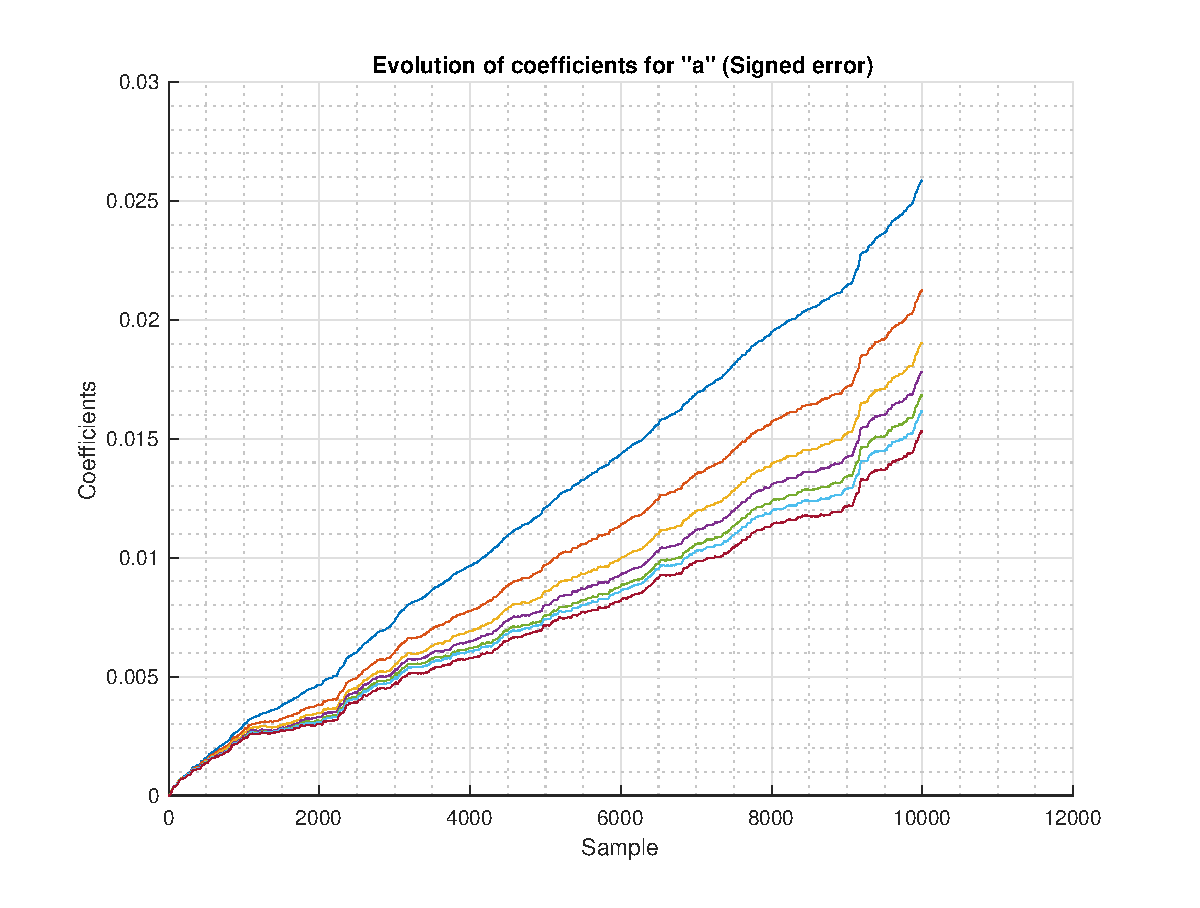
\includegraphics[width = \textwidth]{salg_signerr_sp}
\caption{Signed error}
\label{fig:salg_signerr_ar}
\end{subfigure}
\begin{subfigure}{0.24\textwidth}
\centering
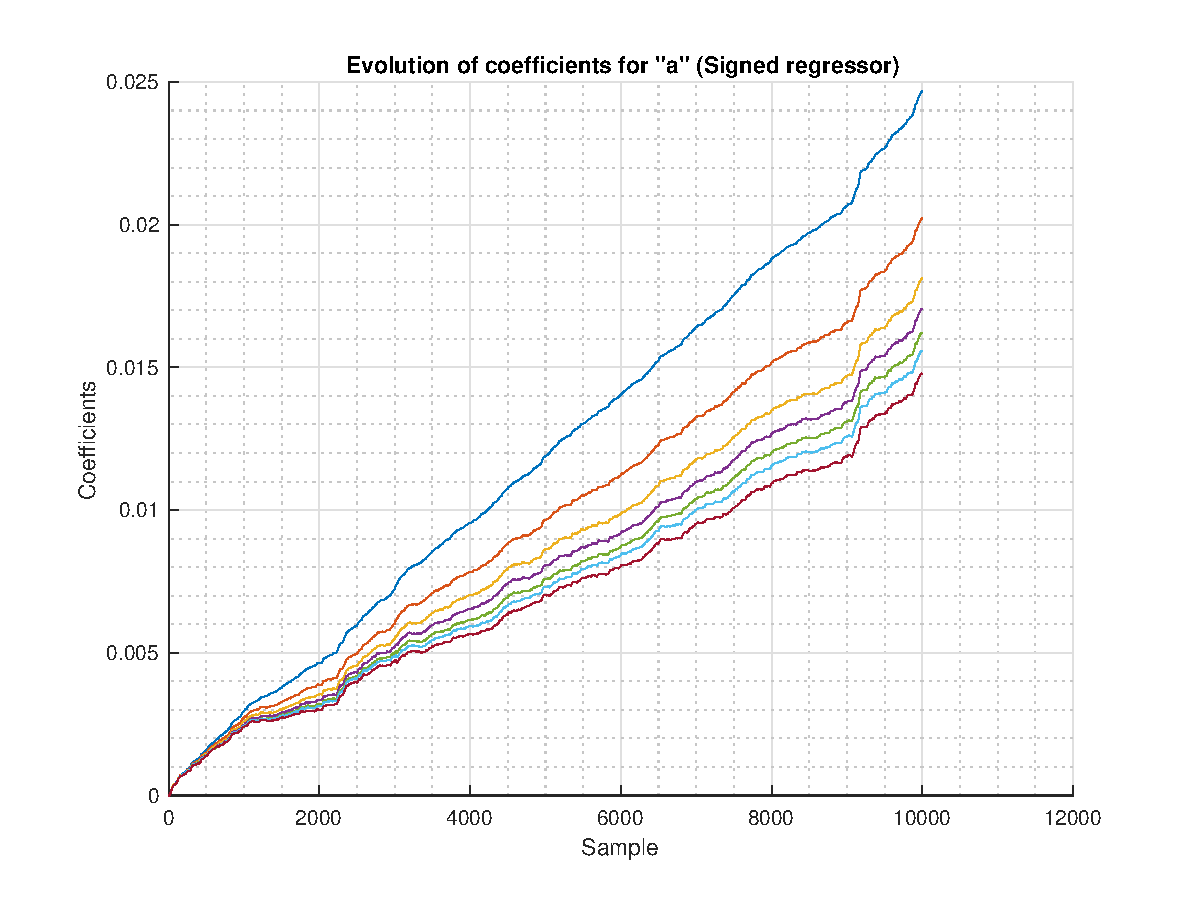
\includegraphics[width = \textwidth]{salg_regressor_sp}
\caption{Signed regressor}
\label{fig:salg_regressor_sp}
\end{subfigure}
\begin{subfigure}{0.24\textwidth}
\centering
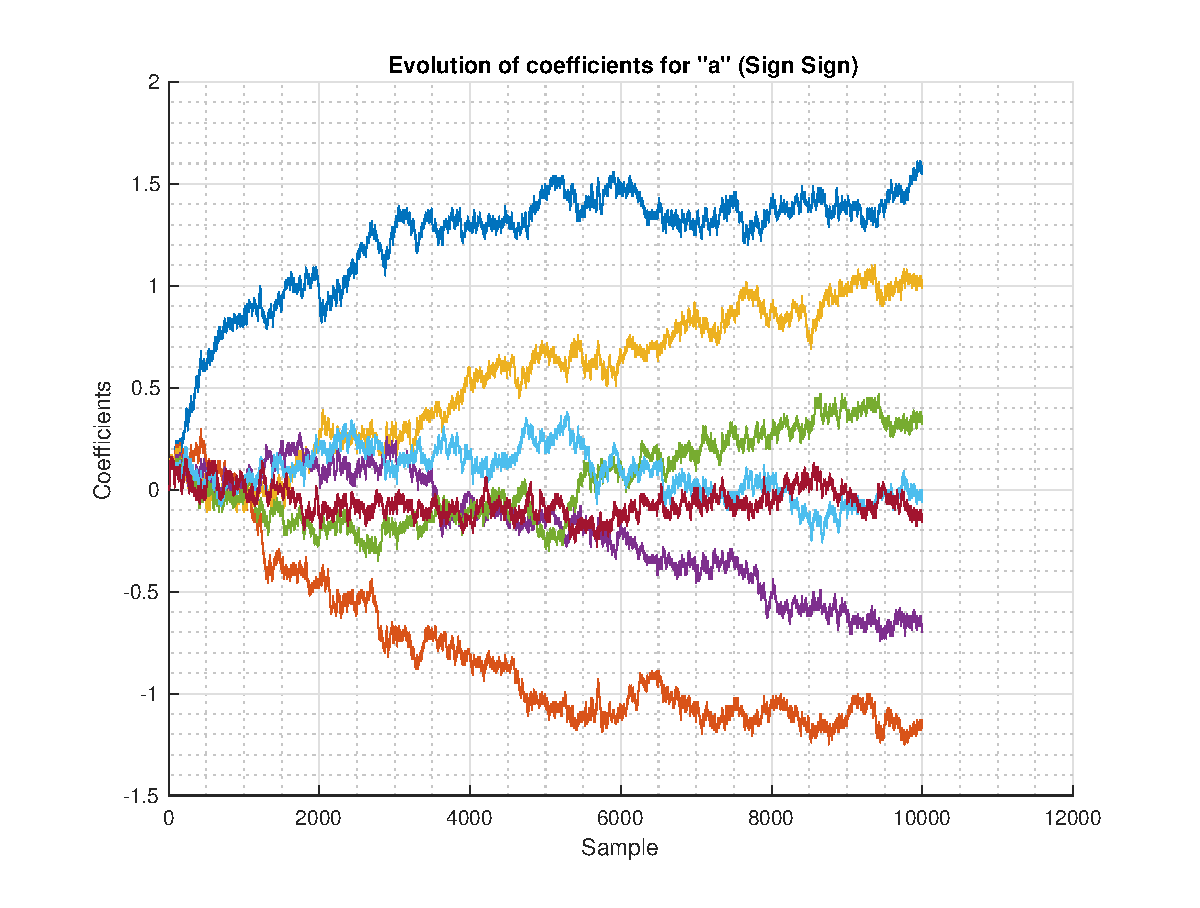
\includegraphics[width = \textwidth]{salg_signsign_sp}
\caption{Sign Sign}
\label{fig:salg_signsign_sp}
\end{subfigure}
\caption{Comparing the performance of signed LMS algorithms for audio signal "a"}
\label{fig:salg_sp}
\end{figure}


\end{document}
